\PassOptionsToPackage{unicode=true}{hyperref} % options for packages loaded elsewhere
\PassOptionsToPackage{hyphens}{url}
%
\documentclass[11pt,ignorenonframetext,]{beamer}
\usepackage{pgfpages}
\setbeamertemplate{caption}[numbered]
\setbeamertemplate{caption label separator}{: }
\setbeamercolor{caption name}{fg=normal text.fg}
\beamertemplatenavigationsymbolsempty
% Prevent slide breaks in the middle of a paragraph:
\widowpenalties 1 10000
\raggedbottom
\setbeamertemplate{part page}{
\centering
\begin{beamercolorbox}[sep=16pt,center]{part title}
  \usebeamerfont{part title}\insertpart\par
\end{beamercolorbox}
}
\setbeamertemplate{section page}{
\centering
\begin{beamercolorbox}[sep=12pt,center]{part title}
  \usebeamerfont{section title}\insertsection\par
\end{beamercolorbox}
}
\setbeamertemplate{subsection page}{
\centering
\begin{beamercolorbox}[sep=8pt,center]{part title}
  \usebeamerfont{subsection title}\insertsubsection\par
\end{beamercolorbox}
}
\AtBeginPart{
  \frame{\partpage}
}
\AtBeginSection{
  \ifbibliography
  \else
    \frame{\sectionpage}
  \fi
}
\AtBeginSubsection{
  \frame{\subsectionpage}
}
\usepackage{lmodern}
\usepackage{amssymb,amsmath}
\usepackage{ifxetex,ifluatex}
\usepackage{fixltx2e} % provides \textsubscript
\ifnum 0\ifxetex 1\fi\ifluatex 1\fi=0 % if pdftex
  \usepackage[T1]{fontenc}
  \usepackage[utf8]{inputenc}
  \usepackage{textcomp} % provides euro and other symbols
\else % if luatex or xelatex
  \usepackage{unicode-math}
  \defaultfontfeatures{Ligatures=TeX,Scale=MatchLowercase}
\fi
\usetheme[]{metropolis}
% use upquote if available, for straight quotes in verbatim environments
\IfFileExists{upquote.sty}{\usepackage{upquote}}{}
% use microtype if available
\IfFileExists{microtype.sty}{%
\usepackage[]{microtype}
\UseMicrotypeSet[protrusion]{basicmath} % disable protrusion for tt fonts
}{}
\IfFileExists{parskip.sty}{%
\usepackage{parskip}
}{% else
\setlength{\parindent}{0pt}
\setlength{\parskip}{6pt plus 2pt minus 1pt}
}
\usepackage{hyperref}
\hypersetup{
            pdftitle={Lecture 11},
            pdfborder={0 0 0},
            breaklinks=true}
\urlstyle{same}  % don't use monospace font for urls
\newif\ifbibliography
\usepackage{color}
\usepackage{fancyvrb}
\newcommand{\VerbBar}{|}
\newcommand{\VERB}{\Verb[commandchars=\\\{\}]}
\DefineVerbatimEnvironment{Highlighting}{Verbatim}{commandchars=\\\{\}}
% Add ',fontsize=\small' for more characters per line
\newenvironment{Shaded}{}{}
\newcommand{\AlertTok}[1]{\textcolor[rgb]{1.00,0.00,0.00}{\textbf{#1}}}
\newcommand{\AnnotationTok}[1]{\textcolor[rgb]{0.38,0.63,0.69}{\textbf{\textit{#1}}}}
\newcommand{\AttributeTok}[1]{\textcolor[rgb]{0.49,0.56,0.16}{#1}}
\newcommand{\BaseNTok}[1]{\textcolor[rgb]{0.25,0.63,0.44}{#1}}
\newcommand{\BuiltInTok}[1]{#1}
\newcommand{\CharTok}[1]{\textcolor[rgb]{0.25,0.44,0.63}{#1}}
\newcommand{\CommentTok}[1]{\textcolor[rgb]{0.38,0.63,0.69}{\textit{#1}}}
\newcommand{\CommentVarTok}[1]{\textcolor[rgb]{0.38,0.63,0.69}{\textbf{\textit{#1}}}}
\newcommand{\ConstantTok}[1]{\textcolor[rgb]{0.53,0.00,0.00}{#1}}
\newcommand{\ControlFlowTok}[1]{\textcolor[rgb]{0.00,0.44,0.13}{\textbf{#1}}}
\newcommand{\DataTypeTok}[1]{\textcolor[rgb]{0.56,0.13,0.00}{#1}}
\newcommand{\DecValTok}[1]{\textcolor[rgb]{0.25,0.63,0.44}{#1}}
\newcommand{\DocumentationTok}[1]{\textcolor[rgb]{0.73,0.13,0.13}{\textit{#1}}}
\newcommand{\ErrorTok}[1]{\textcolor[rgb]{1.00,0.00,0.00}{\textbf{#1}}}
\newcommand{\ExtensionTok}[1]{#1}
\newcommand{\FloatTok}[1]{\textcolor[rgb]{0.25,0.63,0.44}{#1}}
\newcommand{\FunctionTok}[1]{\textcolor[rgb]{0.02,0.16,0.49}{#1}}
\newcommand{\ImportTok}[1]{#1}
\newcommand{\InformationTok}[1]{\textcolor[rgb]{0.38,0.63,0.69}{\textbf{\textit{#1}}}}
\newcommand{\KeywordTok}[1]{\textcolor[rgb]{0.00,0.44,0.13}{\textbf{#1}}}
\newcommand{\NormalTok}[1]{#1}
\newcommand{\OperatorTok}[1]{\textcolor[rgb]{0.40,0.40,0.40}{#1}}
\newcommand{\OtherTok}[1]{\textcolor[rgb]{0.00,0.44,0.13}{#1}}
\newcommand{\PreprocessorTok}[1]{\textcolor[rgb]{0.74,0.48,0.00}{#1}}
\newcommand{\RegionMarkerTok}[1]{#1}
\newcommand{\SpecialCharTok}[1]{\textcolor[rgb]{0.25,0.44,0.63}{#1}}
\newcommand{\SpecialStringTok}[1]{\textcolor[rgb]{0.73,0.40,0.53}{#1}}
\newcommand{\StringTok}[1]{\textcolor[rgb]{0.25,0.44,0.63}{#1}}
\newcommand{\VariableTok}[1]{\textcolor[rgb]{0.10,0.09,0.49}{#1}}
\newcommand{\VerbatimStringTok}[1]{\textcolor[rgb]{0.25,0.44,0.63}{#1}}
\newcommand{\WarningTok}[1]{\textcolor[rgb]{0.38,0.63,0.69}{\textbf{\textit{#1}}}}
\setlength{\emergencystretch}{3em}  % prevent overfull lines
\providecommand{\tightlist}{%
  \setlength{\itemsep}{0pt}\setlength{\parskip}{0pt}}
\setcounter{secnumdepth}{0}

% set default figure placement to htbp
\makeatletter
\def\fps@figure{htbp}
\makeatother

\usepackage{geometry}
\usepackage{graphicx}

\usepackage{bbold}
\usepackage{lmodern}


\usepackage{url}		% produces hyperlinks

\usepackage{colortbl}	% allows for color usage in tables
\usepackage{multirow}	% allows for rows that span multiple rows in tables

\usepackage{color}          	% gives color options
\usepackage{xcolor}		% this package has a variety of color options

\usepackage{multicol}
\usepackage{textcomp}

\usepackage{setspace}
\usepackage{changepage}
\usepackage{isotope}

\singlespacing

\def\begincol{\begin{column}}
\def\endcol{\end{column}}

\def\begincols{\begin{columns}}
\def\endcols{\end{columns}}

%%%%%%%%%%%%%%%%
% Small code output
%%%%%%%%%%%%%%%%

%% change fontsize of R code

\makeatletter
\@ifundefined{Shaded}{\newenvironment{Shaded}{}{}}{}
\makeatother


\let\oldShaded\Shaded
\let\endoldShaded\endShaded
\renewenvironment{Shaded}{\footnotesize\begin{spacing}{0.9}\oldShaded}{\endoldShaded\end{spacing}}

%% change fontsize of output
\let\oldverbatim\verbatim
\let\endoldverbatim\endverbatim
\renewenvironment{verbatim}{\footnotesize\begin{spacing}{0.9}\oldverbatim}{\endoldverbatim\end{spacing}}


\newcommand{\tinyoutput}{
  \renewenvironment{Shaded}{\tiny\begin{spacing}{0.9}\oldShaded}{\endoldShaded\end{spacing}}
  \renewenvironment{verbatim}{\tiny\begin{spacing}{0.9}\oldverbatim}{\endoldverbatim\end{spacing}}
}

\newcommand{\scriptoutput}{
  \renewenvironment{Shaded}{\scriptsize\begin{spacing}{0.9}\oldShaded}{\endoldShaded\end{spacing}}
  \renewenvironment{verbatim}{\scriptsize\begin{spacing}{0.9}\oldverbatim}{\endoldverbatim\end{spacing}}
}

\newcommand{\footnoteoutput}{
  \renewenvironment{Shaded}{\footnotesize\begin{spacing}{0.9}\oldShaded}{\endoldShaded\end{spacing}}
  \renewenvironment{verbatim}{\footnotesize\begin{spacing}{0.9}\oldverbatim}{\endoldverbatim\end{spacing}}
}

%\newcommand{\verbatimfont}[1]{\renewcommand{\verbatim@font}{\ttfamily#1}}


%%%%%%%%%%%%%%%%
% Custom Colors
%%%%%%%%%%%%%%%%

\definecolor{redhl}{rgb}{0.98,0.29,0.28}
\definecolor{yellowhl}{rgb}{0.98,0.87,0.28}


\xdefinecolor{oiBlue}{rgb}{0.15, 0.35, 0.55}
\xdefinecolor{gray}{rgb}{0.5, 0.5, 0.5}
\xdefinecolor{darkGray}{rgb}{0.3, 0.3, 0.3}
\xdefinecolor{darkerGray}{rgb}{0.2, 0.2, 0.2}
\xdefinecolor{rubineRed}{rgb}{0.89,0,0.30}
\xdefinecolor{linkCol}{rgb}{0.11,0.49,0.95}	
\xdefinecolor{irishGreen}{rgb}{0,0.60,0}	
\xdefinecolor{darkturquoise}{rgb}{0.44, 0.58, 0.86}
\definecolor{lightGreen}{rgb}{0.533,0.765,0.42}
%\xdefinecolor{hlblue}{rgb}{0.051,0.65,1}
\xdefinecolor{hlblue}{rgb}{ 0.055, 0.639, 0.831}
\definecolor{light}{rgb}{.337,.608,.741}
\definecolor{dark}{rgb}{.337,.608,.741}

\definecolor{cpink}{rgb}{0.93, 0.23, 0.51}

%%%%%%%%%%%%%%%%
% Custom Commands
%%%%%%%%%%%%%%%%

% text colors
\newcommand{\red}[1]{\textit{\textcolor{rubineRed}{#1}}}
\newcommand{\orange}[1]{\textit{\textcolor{orange}{#1}}}
\newcommand{\pink}[1]{\textit{\textcolor{rubineRed!90!white!50}{#1}}}
\newcommand{\green}[1]{\textit{\textcolor{irishGreen}{#1}}}
\newcommand{\blue}[1]{\textit{\textcolor{darkturquoise}{#1}}}
\newcommand{\light}[1]{\textcolor{light}{\textbf{#1}}}
\newcommand{\dark}[1]{\textcolor{dark}{#1}}
\newcommand{\gray}[1]{\textcolor{gray}{#1}}


% mail
\newcommand{\mail}[1]{\href{mailto:#1}{\textit{\textcolor{linkCol}{#1}}}}

% highlighting: hl, hlGr, mathhl
\newcommand{\hl}[1]{\textit{\textcolor{hlblue}{#1}}}
\newcommand{\hlGr}[1]{\textit{\textcolor{lightGreen}{#1}}}
\newcommand{\hlRd}[1]{\textit{\textcolor{rubineRed}{#1}}}
\newcommand{\mathhl}[1]{\textcolor{hlblue}{\ensuremath{#1}}}
\newcommand{\hlr}[1]{\fcolorbox{redhl}{white}{$\displaystyle #1$}}
\newcommand{\hly}[1]{\fcolorbox{yellowhl}{white}{$\displaystyle #1$}}


\newcommand{\vvfill}{\vskip0pt plus 1filll}

\DeclareMathOperator*{\argmin}{arg\,min}
\DeclareMathOperator*{\argmax}{arg\,max}

\title{Lecture 11}
\providecommand{\subtitle}[1]{}
\subtitle{Fitting ARIMA Models}
\date{10/10/2018}

\begin{document}
\frame{\titlepage}

\hypertarget{model-fitting}{%
\section{Model Fitting}\label{model-fitting}}

\begin{frame}[t]{Fitting ARIMA}
\protect\hypertarget{fitting-arima}{}

For an \(ARIMA(p,d,q)\) model

\begin{itemize}
\item
  Requires that the data be stationary after differencing \vspace{3mm}
\item
  Handling \(d\) is straight forward, just difference the original data
  \(d\) times (leaving \(n-d\) observations)
  \[ y'_t = \Delta^d \, y_t \] \vspace{3mm}
\item
  After differencing, fit an \(ARMA(p,q)\) model to \(y'_t\).
  \vspace{3mm}
\item
  To keep things simple we'll assume
  \(w_t \overset{iid}{\sim} \mathcal{N}(0,\sigma^2_w)\)
\end{itemize}

\end{frame}

\begin{frame}{MLE - Stationarity \& iid normal errors}
\protect\hypertarget{mle---stationarity-iid-normal-errors}{}

If both of these conditions are met, then the time series \(y_t\) will
also be normal.

\pause

\(~\)

In general, the vector \(\symbf{y} = (y_1, y_2, \ldots, y_t)'\) will
have a multivariate normal distribution with mean
\(\{\symbf\mu\}_i = E(y_i) = E(y_t)\) and covariance \(\symbf\Sigma\)
where \(\{\symbf{\Sigma}\}_{ij} = \gamma(i-j)\).

\(~\)

The joint density of \(\symbf y\) is given by

\[ f_{\symbf y}(\symbf y) = \frac{1}{(2\pi)^{t/2}\,\det(\symbf\Sigma)^{1/2}} \times \exp\left( -\frac{1}{2}(\symbf y - \symbf \mu)' \, \Sigma^{-1} \, (\symbf y - \symbf \mu) \right) \]

\end{frame}

\hypertarget{ar}{%
\section{AR}\label{ar}}

\begin{frame}[t]{Fitting \(AR(1)\)}
\protect\hypertarget{fitting-ar1}{}

\[ y_t = \delta + \phi \, y_{t-1} + w_t \]

We need to estimate three parameters: \(\delta\), \(\phi\), and
\(\sigma_w^2\), we know

\[ 
\begin{aligned}
E(y_t) &= \frac{\delta}{1-\phi} \\
Var(y_t) &= \frac{\sigma_w^2}{1-\phi^2} \\
\gamma_h &= \frac{\sigma_w^2}{1-\phi^2} \phi^{|h|}
\end{aligned} 
\]

Using these properties it is possible to write the distribution of
\(\symbf{y}\) as a MVN but that does not make it easy to write down a
(simplified) closed form for the MLE estimate for \(\delta\), \(\phi\),
and \(\sigma_w^2\).

\end{frame}

\begin{frame}{Conditional Density}
\protect\hypertarget{conditional-density}{}

We can also rewrite the density as follows,

\[
\begin{aligned}
f_{\symbf y}
  &= f_{y_t,\,y_{t-1},\,\ldots,\,y_2,\,y_1} \\
  &= f_{y_t|\,y_{t-1},\,\ldots,\,y_2,\,y_1} f_{y_{t-1}|y_{t-2},\,\ldots,\,y_2,\,y_1} \cdots f_{y_2|y_1} f_{y_1} \\
  &= f_{y_t|\,y_{t-1}} f_{y_{t-1}|y_{t-2}} \cdots f_{y_2|y_1} f_{y_1} 
\end{aligned}
\]

where,

\[
\begin{aligned}
y_1 &\sim \mathcal{N}\left(\delta, \, \frac{\sigma^2_w}{1-\phi^2} \right) \\
y_{t}|y_{t-1} &\sim \mathcal{N}\left(\delta+\phi\, y_{t-1}, \, \sigma^2_w \right) \\
f_{y_{t}|y_{t-1}}(y_t) &= \frac{1}{\sqrt{2\pi \, \sigma^2_w}} \exp \left( -\frac{1}{2}\frac{(y_t -\delta+\phi\, y_{t-1})^2 }{\sigma^2_w} \right)
\end{aligned}
\]

\end{frame}

\begin{frame}[t]{Log likelihood of AR(1)}
\protect\hypertarget{log-likelihood-of-ar1}{}

\scriptsize

\[
\log f_{y_{t} | y_{t-1}}(y_t) = -\frac{1}{2}\left( \log 2\pi + \log \sigma^2_w + \frac{1}{\sigma_w^2} (y_t -\delta+\phi\, y_{t-1})^2 \right)
\]

\[
\begin{aligned}
\ell(\delta, \phi, \sigma^2_w) 
  &= \log f_{\symbf{y}} = \log f_{y_1} + \sum_{i=2}^t \log f_{y_{i}|y_{i-1}} \\
  &= - \frac{1}{2} \bigg(\log 2\pi + \log \sigma_w^2 - \log (1-\phi^2) + \frac{(1-\phi^2)}{\sigma_w^2 }(y_1-\delta)^2 \bigg) \\
  & ~~~~ - \frac{1}{2} \bigg( (n-1) \log 2\pi + (n-1) \log \sigma_w^2 + \frac{1}{\sigma_w^2} \sum_{i=2}^n (y_i -\delta+\phi\, y_{i-1})^2 \bigg) \\
  &= - \frac{1}{2} \bigg( n \log 2\pi + n \log \sigma_w^2 - \log (1-\phi^2) \\
  &~~~~~~~~~~~~~~~+ \frac{1}{\sigma_w^2} \bigg( (1-\phi^2)(y_1-\delta)^2 + \sum_{i=2}^n (y_i -\delta+\phi\, y_{i-1})^2 \bigg) \bigg)
\end{aligned}
\]

\end{frame}

\begin{frame}[t]{AR(1) Example}
\protect\hypertarget{ar1-example}{}

with \(\phi = 0.75\), \(\delta=0.5\), and \(\sigma_w^2=1\),

\begin{center}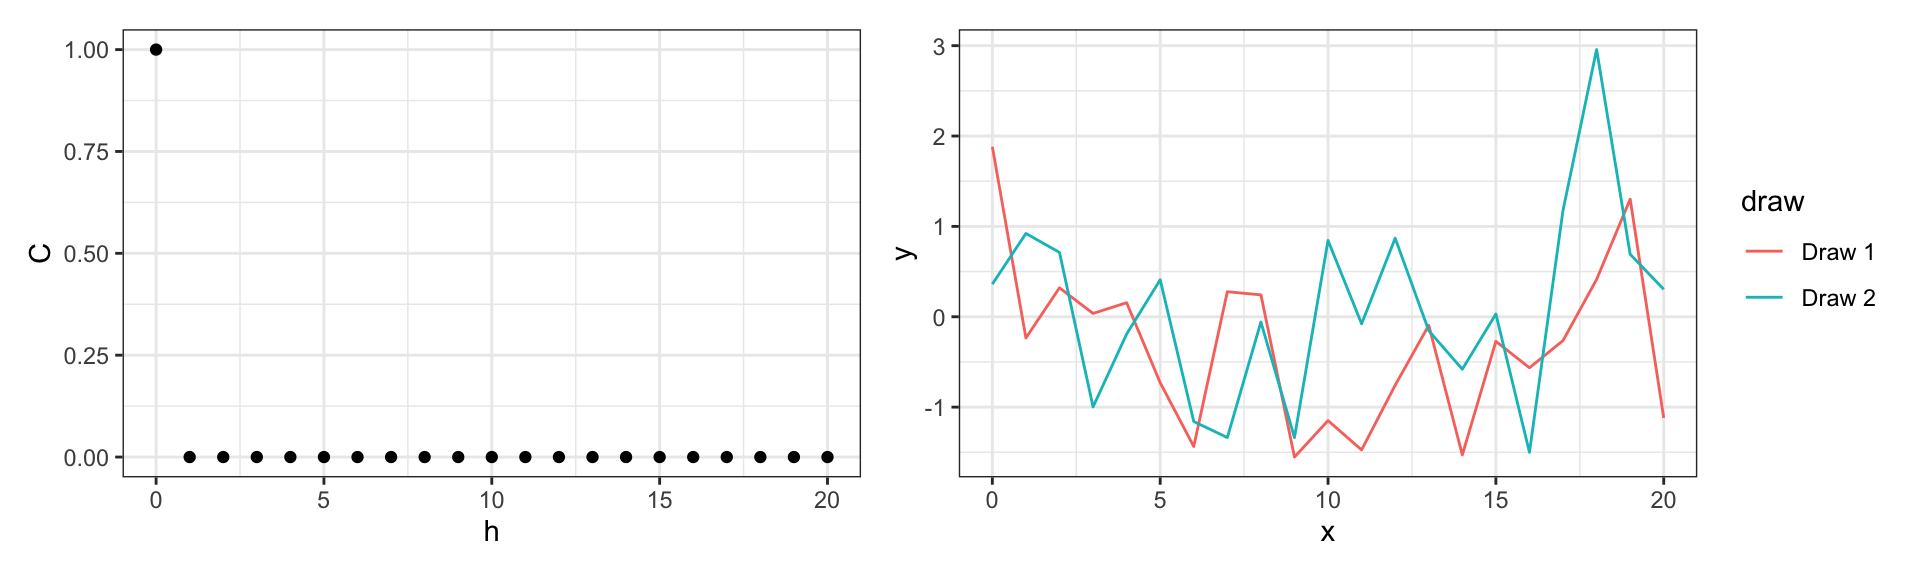
\includegraphics[width=\textwidth]{Lec11_files/figure-beamer/unnamed-chunk-1-1} \end{center}

\end{frame}

\begin{frame}[fragile,t]{Arima}
\protect\hypertarget{arima}{}

\begin{Shaded}
\begin{Highlighting}[]
\NormalTok{ar1_arima =}\StringTok{ }\NormalTok{forecast}\OperatorTok{::}\KeywordTok{Arima}\NormalTok{(ar1, }\DataTypeTok{order =} \KeywordTok{c}\NormalTok{(}\DecValTok{1}\NormalTok{,}\DecValTok{0}\NormalTok{,}\DecValTok{0}\NormalTok{)) }
\KeywordTok{summary}\NormalTok{(ar1_arima)}
\CommentTok{## Series: ar1 }
\CommentTok{## ARIMA(1,0,0) with non-zero mean }
\CommentTok{## }
\CommentTok{## Coefficients:}
\CommentTok{##          ar1    mean}
\CommentTok{##       0.7312  1.8934}
\CommentTok{## s.e.  0.0309  0.1646}
\CommentTok{## }
\CommentTok{## sigma^2 estimated as 0.994:  log likelihood=-707.35}
\CommentTok{## AIC=1420.71   AICc=1420.76   BIC=1433.35}
\CommentTok{## }
\CommentTok{## Training set error measures:}
\CommentTok{##                       ME      RMSE       MAE       MPE     MAPE      MASE}
\CommentTok{## Training set 0.005333274 0.9950158 0.7997576 -984.9413 1178.615 0.9246146}
\CommentTok{##                     ACF1}
\CommentTok{## Training set -0.04437489}
\end{Highlighting}
\end{Shaded}

\end{frame}

\begin{frame}[fragile,t]{lm}
\protect\hypertarget{lm}{}

\begin{Shaded}
\begin{Highlighting}[]
\NormalTok{d =}\StringTok{ }\KeywordTok{data_frame}\NormalTok{(}\DataTypeTok{y =}\NormalTok{ ar1 }\OperatorTok\StringTok{ }\KeywordTok{strip_attrs}\NormalTok{(), }\DataTypeTok{t=}\KeywordTok{seq_along}\NormalTok{(ar1))}
\NormalTok{ar1_lm =}\StringTok{ }\KeywordTok{lm}\NormalTok{(y}\OperatorTok{~}\KeywordTok{lag}\NormalTok{(y), }\DataTypeTok{data=}\NormalTok{d)}
\KeywordTok{summary}\NormalTok{(ar1_lm)}
\CommentTok{## }
\CommentTok{## Call:}
\CommentTok{## lm(formula = y ~ lag(y), data = d)}
\CommentTok{## }
\CommentTok{## Residuals:}
\CommentTok{##     Min      1Q  Median      3Q     Max }
\CommentTok{## -3.2772 -0.6880  0.0785  0.6819  2.5704 }
\CommentTok{## }
\CommentTok{## Coefficients:}
\CommentTok{##             Estimate Std. Error t value Pr(>|t|)    }
\CommentTok{## (Intercept)  0.52347    0.07328   7.144 3.25e-12 ***}
\CommentTok{## lag(y)       0.72817    0.03093  23.539  < 2e-16 ***}
\CommentTok{## ---}
\CommentTok{## Signif. codes:  0 '***' 0.001 '**' 0.01 '*' 0.05 '.' 0.1 ' ' 1}
\CommentTok{## }
\CommentTok{## Residual standard error: 0.9949 on 497 degrees of freedom}
\CommentTok{##   (1 observation deleted due to missingness)}
\CommentTok{## Multiple R-squared:  0.5272, Adjusted R-squared:  0.5262 }
\CommentTok{## F-statistic: 554.1 on 1 and 497 DF,  p-value: < 2.2e-16}
\end{Highlighting}
\end{Shaded}

\end{frame}

\begin{frame}[fragile,t]{Bayesian AR(1) Model}
\protect\hypertarget{bayesian-ar1-model}{}

\begin{Shaded}
\begin{Highlighting}[]
\NormalTok{ar1_model =}\StringTok{ "model\{}
\StringTok{# likelihood}
\StringTok{  y[1] ~ dnorm(delta/(1-phi), (sigma2_w/(1-phi^2))^-1)}
\StringTok{  y_hat[1] ~ dnorm(delta/(1-phi), (sigma2_w/(1-phi^2))^-1)}

\StringTok{  for (t in 2:length(y)) \{}
\StringTok{    y[t] ~ dnorm(delta + phi*y[t-1], 1/sigma2_w)}
\StringTok{    y_hat[t] ~ dnorm(delta + phi*y[t-1], 1/sigma2_w)}
\StringTok{  \}}
\StringTok{  }
\StringTok{  mu = delta/(1-phi)}

\StringTok{# priors}
\StringTok{  delta ~ dnorm(0,1/1000)}
\StringTok{  phi ~ dnorm(0,1)}
\StringTok{  tau ~ dgamma(0.001,0.001)}
\StringTok{  sigma2_w <- 1/tau}
\StringTok{\}"}
\end{Highlighting}
\end{Shaded}

\end{frame}

\begin{frame}{Chains}
\protect\hypertarget{chains}{}

\begin{center}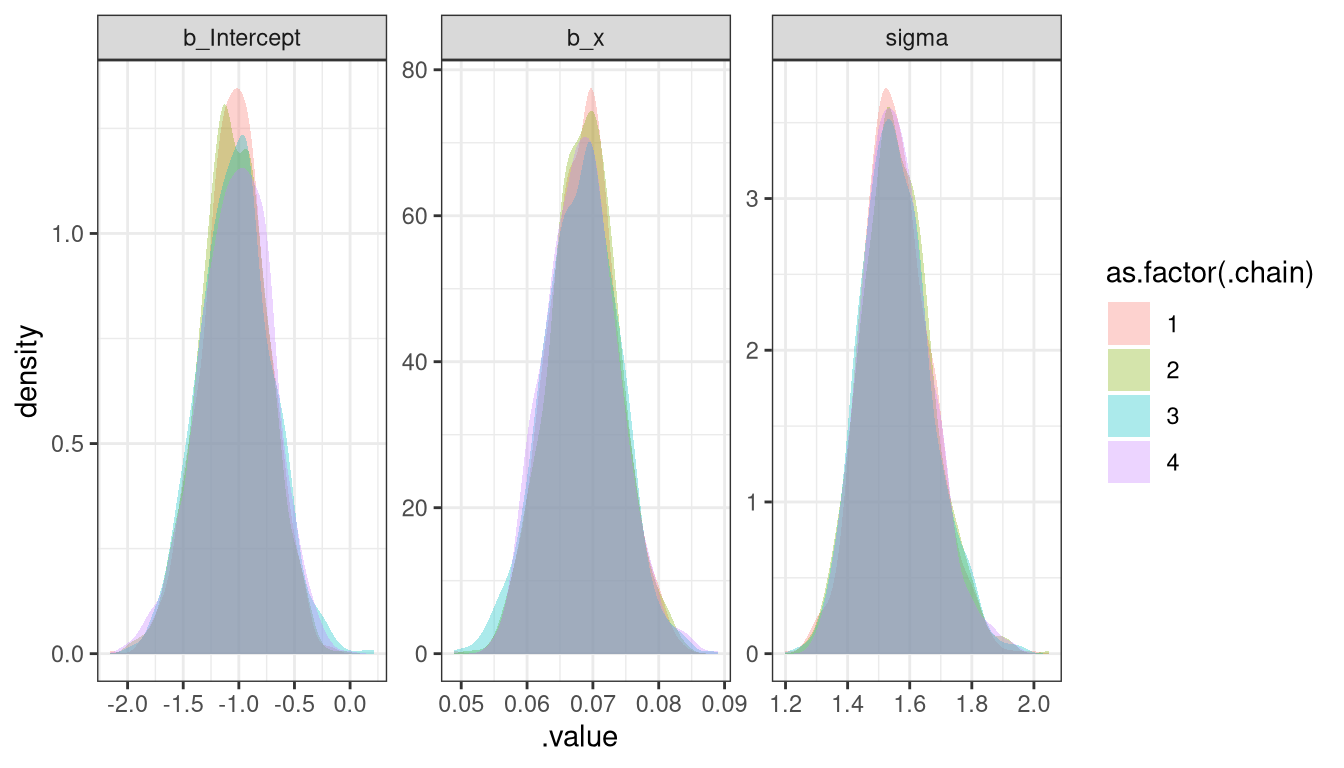
\includegraphics[width=\textwidth]{Lec11_files/figure-beamer/unnamed-chunk-7-1} \end{center}

\end{frame}

\begin{frame}{Posteriors}
\protect\hypertarget{posteriors}{}

\begin{center}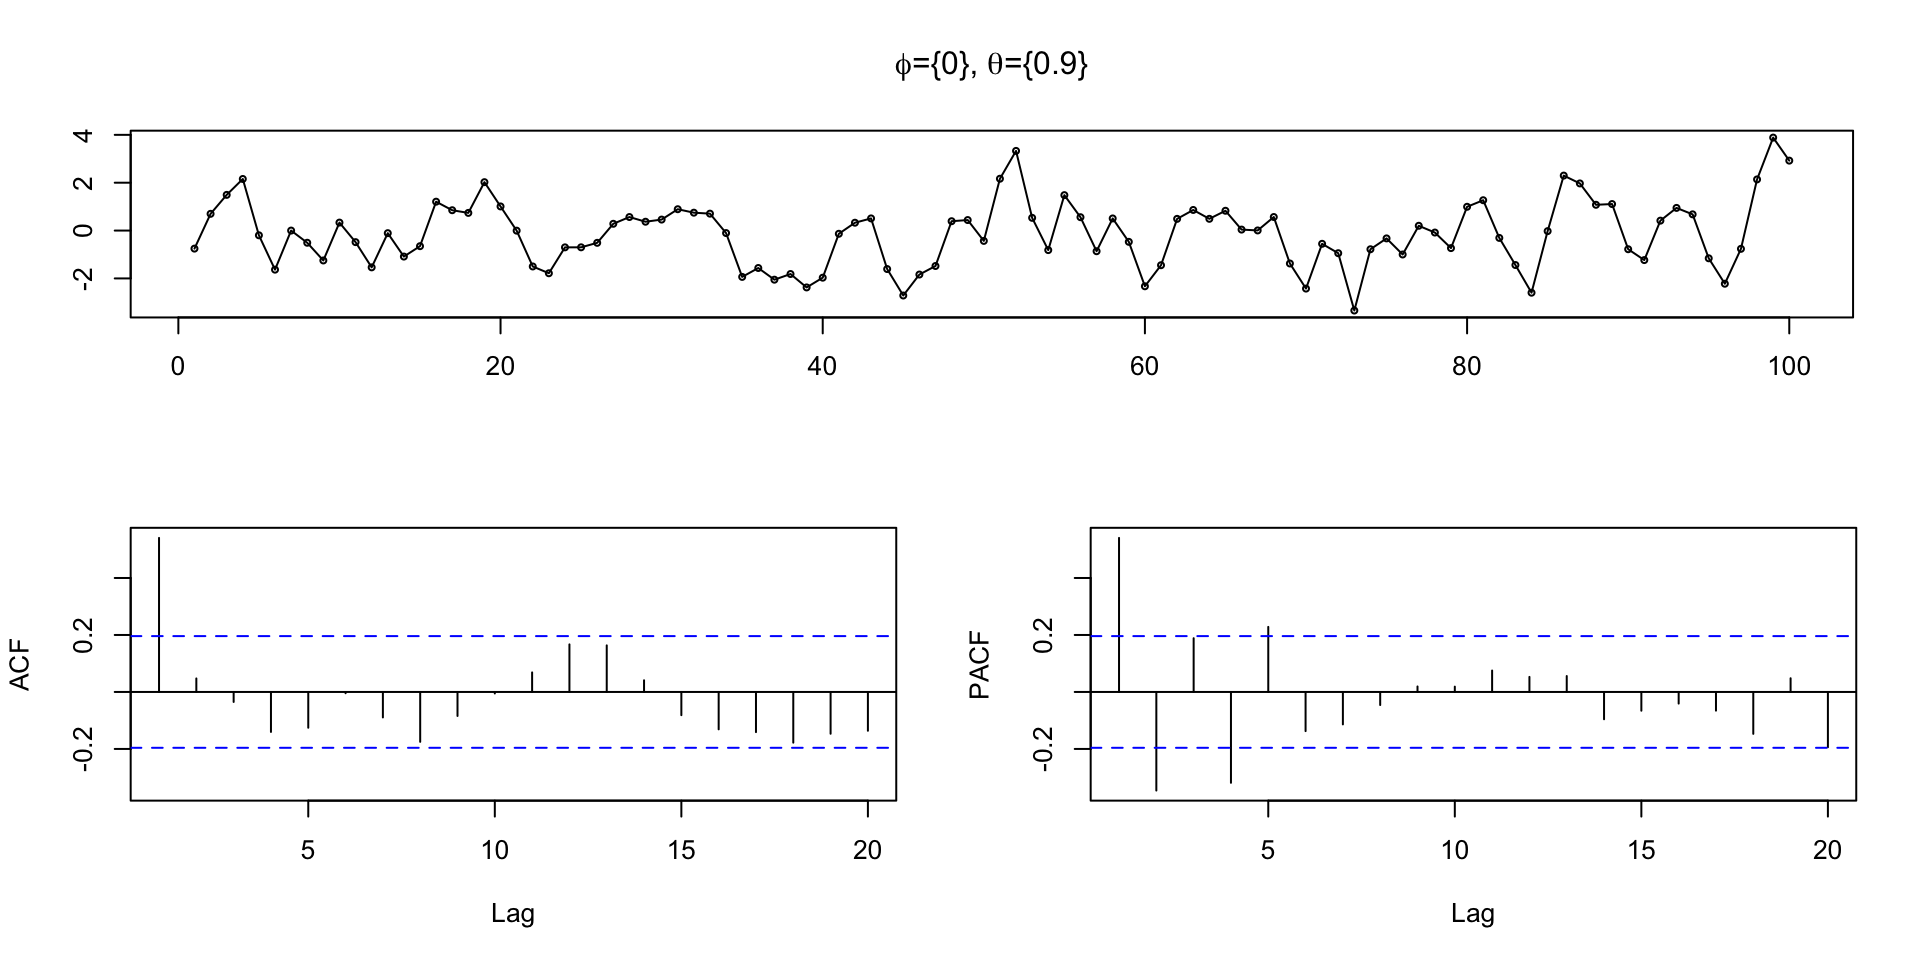
\includegraphics[width=\textwidth]{Lec11_files/figure-beamer/unnamed-chunk-8-1} \end{center}

\end{frame}

\begin{frame}{Predictions}
\protect\hypertarget{predictions}{}

\begin{center}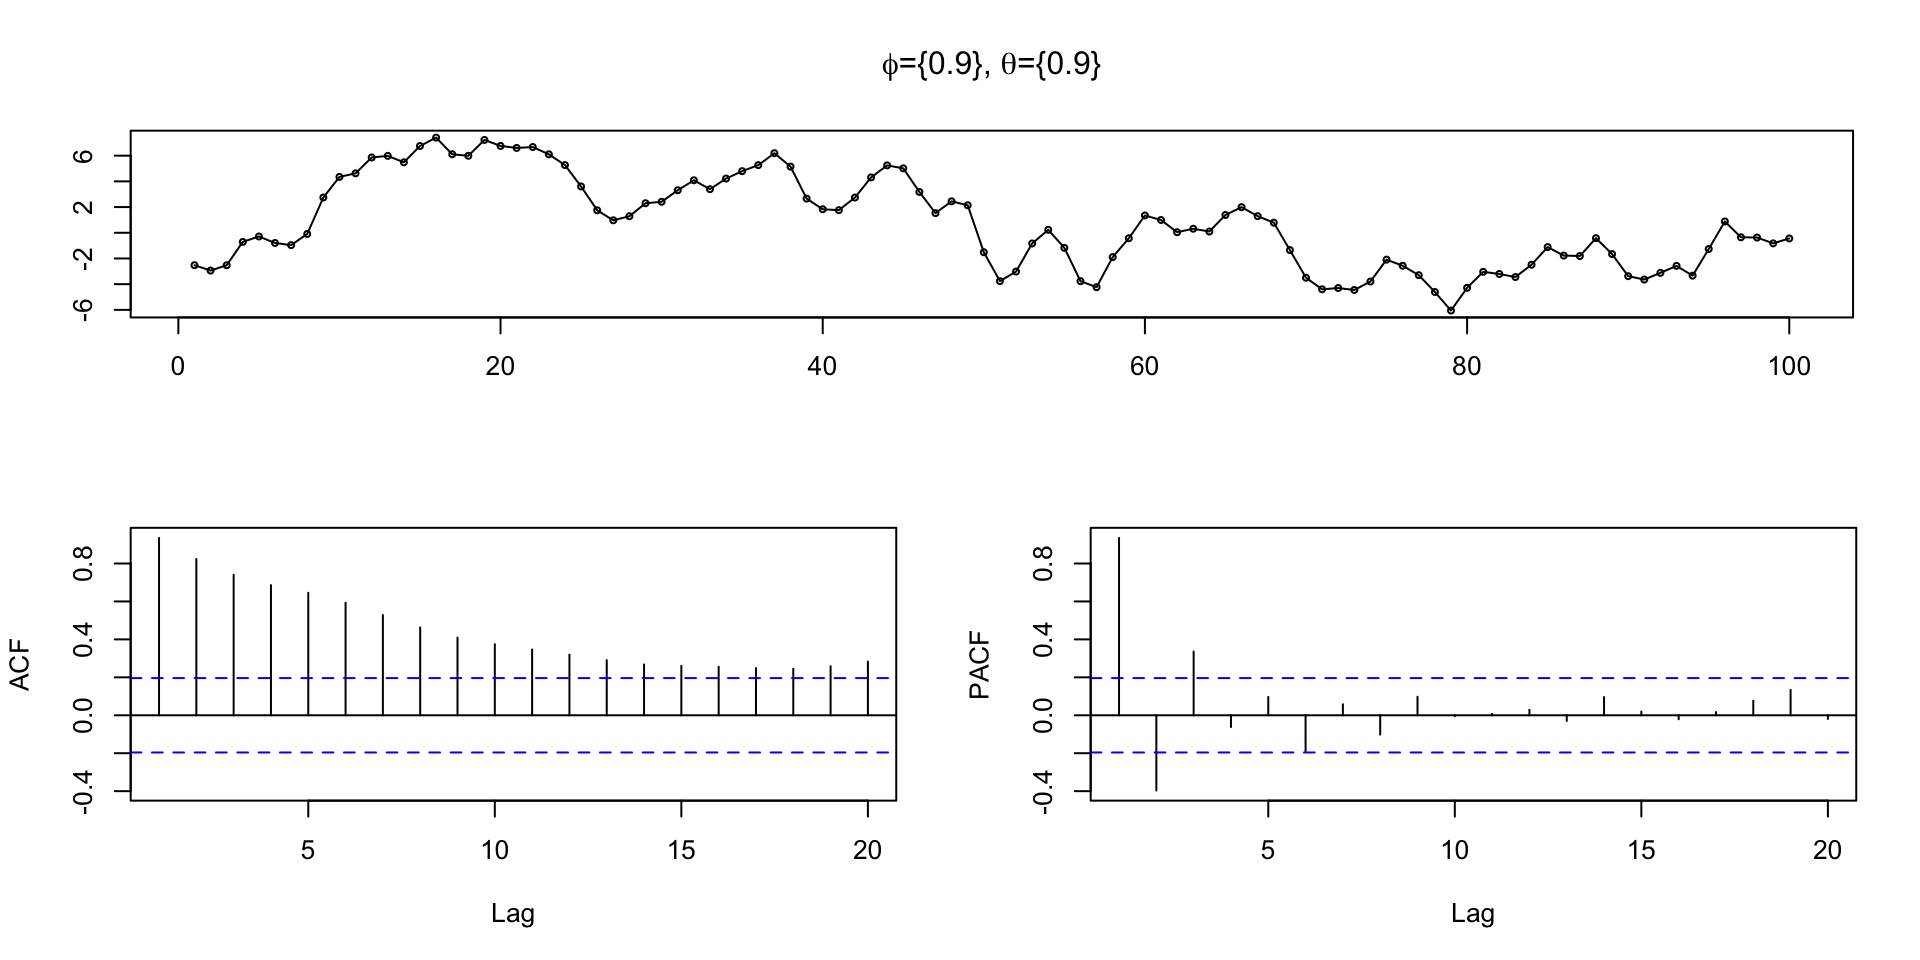
\includegraphics[width=\textwidth]{Lec11_files/figure-beamer/unnamed-chunk-9-1} \end{center}

\end{frame}

\begin{frame}{Faceted}
\protect\hypertarget{faceted}{}

\begin{center}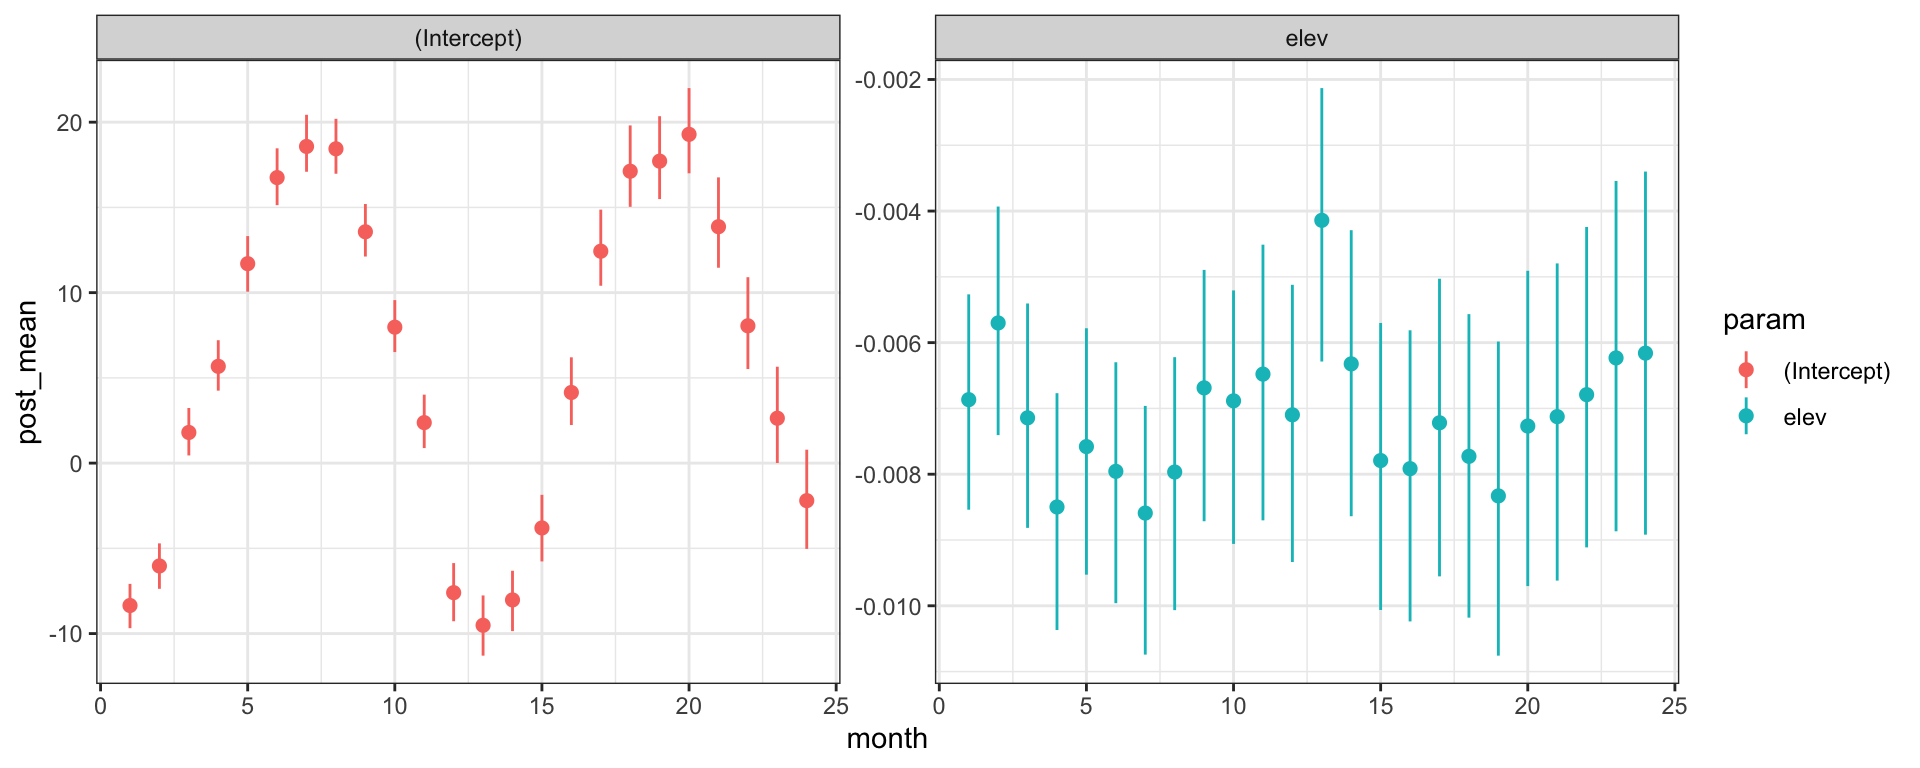
\includegraphics[width=\textwidth]{Lec11_files/figure-beamer/unnamed-chunk-10-1} \end{center}

\end{frame}

\begin{frame}[t]{Fitting AR(p) - Lagged Regression}
\protect\hypertarget{fitting-arp---lagged-regression}{}

We can rewrite the density as follows, \[
\begin{aligned}
f(\symbf y)
  &= f(y_t, \,y_{t-1}, \,\ldots, \,y_{2}, \,y_{1}) \\
  &= f(y_{n}|y_{n-1},\ldots,y_{n-p}) \cdots  f(y_{p+1}|y_p,\ldots,y_1)  f(y_p, \,\ldots, y_1)
\end{aligned}
\]

\pause

Regressing \(y_t\) on \(y_{t-p}, \ldots, y_{t-1}\) gets us an
approximate solution, but it ignores the
\(f(y_1, \, y_2, \,\ldots, y_p)\) part of the likelihood.

How much does this matter (vs.~using the full likelihood)?

\begin{itemize}
\item
  If \(p\) is near to \(n\) then probably a lot
\item
  If \(p << n\) then probably not much
\end{itemize}

\end{frame}

\begin{frame}[t]{Fitting AR(p) - Method of Moments}
\protect\hypertarget{fitting-arp---method-of-moments}{}

Recall for an AR(p) process,

\[
\begin{aligned}
\gamma(0) &= \sigma^2_w + \phi_1 \gamma(1) + \phi_2 \gamma(2) + \ldots + \phi_p \gamma(p) \\
\gamma(h) &= \phi_1 \gamma(h-1) + \phi_2 \gamma(h-2) + \ldots \phi_p \gamma(h-p)
\end{aligned}
\] We can rewrite the first equation in terms of \(\sigma^2_w\), \[
\sigma^2_w =  \gamma(0) - \phi_1 \gamma(1) - \phi_2 \gamma(2) - \ldots - \phi_p \gamma(p)
\] these are called the Yule-Walker equations.

\end{frame}

\begin{frame}[t]{Yule-Walker}
\protect\hypertarget{yule-walker}{}

These equations can be rewritten into matrix notation as follows

\[
\underset{p \times p}{\symbf\Gamma_p} \underset{p \times 1}{\symbf\phi} = \underset{p \times 1}{\symbf\gamma_p}
\qquad\qquad
\underset{1 \times 1}{\sigma^2_w} = \underset{1 \times 1}{\gamma(0)} - \underset{1 \times p}{\symbf{\phi'}}\underset{p \times 1}{\symbf{\gamma_p}}
\] where \[ 
\begin{aligned}
\underset{p \times p}{\symbf{\Gamma_p}} &= \{\gamma(j-k)\}_{j,k} \\
\underset{p \times 1}{\symbf\phi} &= (\phi_1, \phi_2, \ldots, \phi_p)' \\
\underset{p \times 1}{\symbf\gamma_p} &= (\gamma(1), \gamma(2), \ldots, \gamma(p))'
\end{aligned}
\]

\pause

If we estimate the covariance structure from the data we obtain
\(\hat{\symbf\gamma_p}\) which can plug in and solve for
\(\symbf{\phi}\) and \(\sigma^2_w\), \[
\hat{\symbf\phi} =\hat{\symbf{\Gamma}_p}^{-1}\hat{\symbf{\gamma}_p}
\qquad\qquad
\sigma^2_w = \gamma(0) - \hat{\symbf{\gamma}_p}' \hat{\symbf{\Gamma}_p^{-1}} \hat{\symbf{\gamma}_p}
\]

\end{frame}

\hypertarget{arma}{%
\section{ARMA}\label{arma}}

\begin{frame}[t]{Fitting \(ARMA(2,2)\)}
\protect\hypertarget{fitting-arma22}{}

\[ y_t = \delta + \phi_1 \, y_{t-1} + \phi_2 \, y_{t-2} + \theta_1 w_{t-1} + \theta_2 w_{t-2} + w_t \]

Need to estimate six parameters: \(\delta\), \(\phi_1\), \(\phi_2\),
\(\theta_1\), \(\theta_2\) and \(\sigma_w^2\).

\pause

\(~\)

We could figure out \(E(y_t)\), \(Var(y_t)\), and \(Cov(y_t, y_{t+h})\),
but the last two are going to be pretty nasty and the full MVN likehood
is similarly going to be unpleasant to work with.

\pause

\(~\)

Like the AR(1) and AR(p) processes we want to use conditioning to
simplify things. \tinyoutput \[
\begin{aligned}
y_t | \delta, &y_{t-1}, y_{t-2}, w_{t-1}, w_{t-2} \\ 
&\sim \mathcal{N}(\delta + \phi_1 \, y_{t-1} + \phi_2 \, y_{t-2} + \theta_1 w_{t-1} + \theta_2 w_{t-2},~\sigma_w^2) 
\end{aligned}
\]

\end{frame}

\begin{frame}{ARMA(2,2) Example}
\protect\hypertarget{arma22-example}{}

with \(\phi = (1.3,-0.5)\), \(\theta = (0.5,0.2)\), \(\delta=0\), and
\(\sigma_w^2=1\) using the same models

\begin{center}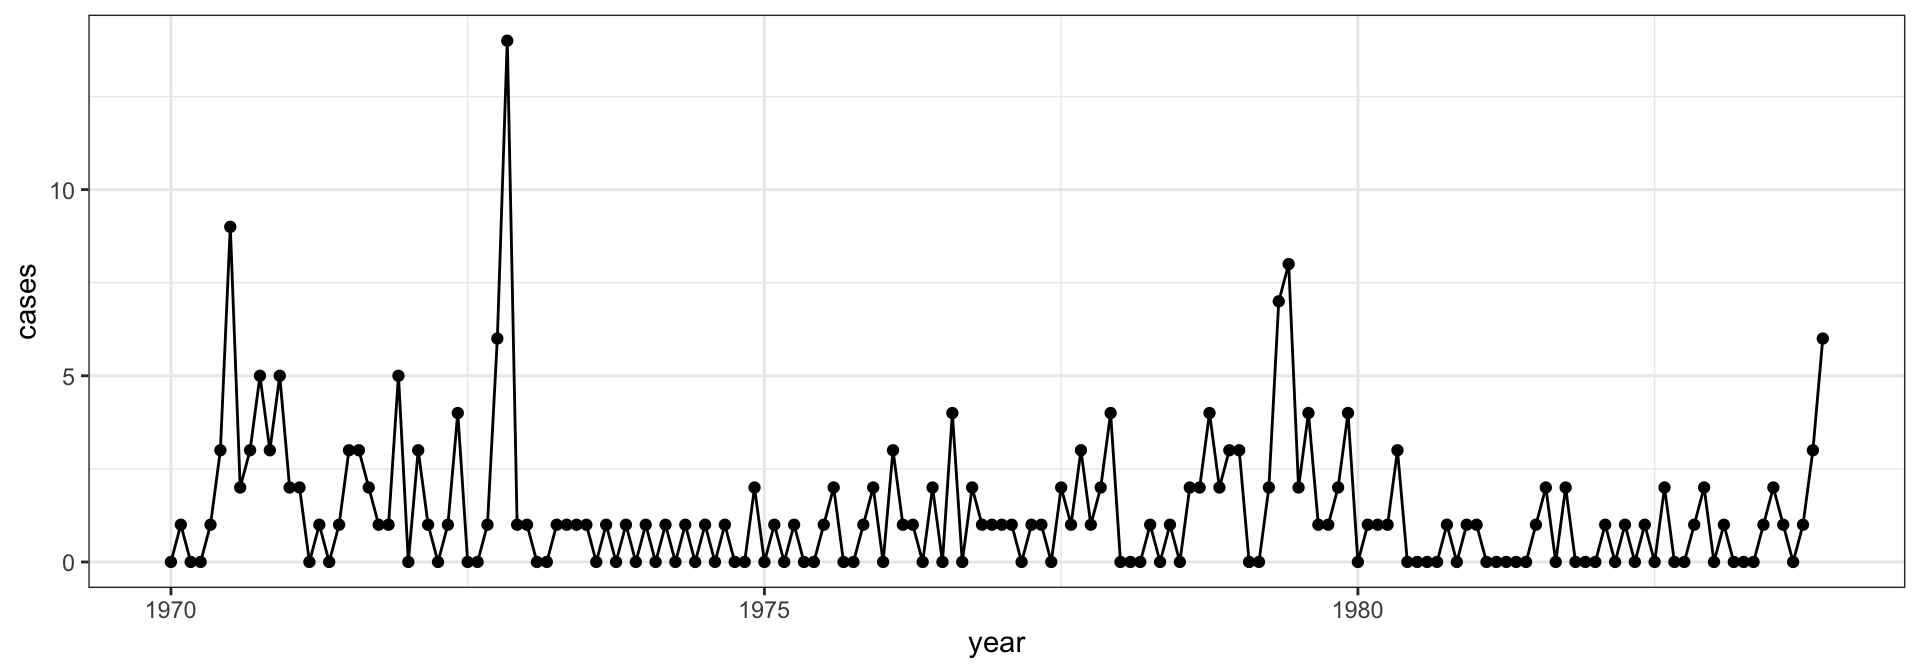
\includegraphics[width=\textwidth]{Lec11_files/figure-beamer/unnamed-chunk-11-1} \end{center}

\end{frame}

\begin{frame}[fragile]{ARIMA}
\protect\hypertarget{arima-1}{}

\begin{Shaded}
\begin{Highlighting}[]
\NormalTok{forecast}\OperatorTok{::}\KeywordTok{Arima}\NormalTok{(y, }\DataTypeTok{order =} \KeywordTok{c}\NormalTok{(}\DecValTok{2}\NormalTok{,}\DecValTok{0}\NormalTok{,}\DecValTok{2}\NormalTok{), }\DataTypeTok{include.mean =} \OtherTok{FALSE}\NormalTok{) }\OperatorTok\StringTok{ }\KeywordTok{summary}\NormalTok{()}
\CommentTok{## Series: y }
\CommentTok{## ARIMA(2,0,2) with zero mean }
\CommentTok{## }
\CommentTok{## Coefficients:}
\CommentTok{##          ar1      ar2     ma1     ma2}
\CommentTok{##       1.2318  -0.4413  0.5888  0.2400}
\CommentTok{## s.e.  0.0843   0.0767  0.0900  0.0735}
\CommentTok{## }
\CommentTok{## sigma^2 estimated as 0.9401:  log likelihood=-693.82}
\CommentTok{## AIC=1397.64   AICc=1397.77   BIC=1418.72}
\CommentTok{## }
\CommentTok{## Training set error measures:}
\CommentTok{##                      ME     RMSE       MAE      MPE     MAPE      MASE}
\CommentTok{## Training set 0.00952552 0.965688 0.7680317 14.16358 142.9927 0.6321085}
\CommentTok{##                       ACF1}
\CommentTok{## Training set -0.0007167096}
\end{Highlighting}
\end{Shaded}

\end{frame}

\begin{frame}[fragile]{AR only lm}
\protect\hypertarget{ar-only-lm}{}

\begin{Shaded}
\begin{Highlighting}[]
\KeywordTok{lm}\NormalTok{(y }\OperatorTok{~}\StringTok{ }\KeywordTok{lag}\NormalTok{(y,}\DecValTok{1}\NormalTok{) }\OperatorTok{+}\StringTok{ }\KeywordTok{lag}\NormalTok{(y,}\DecValTok{2}\NormalTok{)) }\OperatorTok\StringTok{ }\KeywordTok{summary}\NormalTok{()}
\CommentTok{## }
\CommentTok{## Call:}
\CommentTok{## lm(formula = y ~ lag(y, 1) + lag(y, 2))}
\CommentTok{## }
\CommentTok{## Residuals:}
\CommentTok{##     Min      1Q  Median      3Q     Max }
\CommentTok{## -2.7407 -0.6299  0.0012  0.7195  3.2872 }
\CommentTok{## }
\CommentTok{## Coefficients:}
\CommentTok{##             Estimate Std. Error t value Pr(>|t|)    }
\CommentTok{## (Intercept)  0.01196    0.04600    0.26    0.795    }
\CommentTok{## lag(y, 1)    1.57234    0.03057   51.43   <2e-16 ***}
\CommentTok{## lag(y, 2)   -0.73298    0.03059  -23.96   <2e-16 ***}
\CommentTok{## ---}
\CommentTok{## Signif. codes:  0 '***' 0.001 '**' 0.01 '*' 0.05 '.' 0.1 ' ' 1}
\CommentTok{## }
\CommentTok{## Residual standard error: 1.026 on 495 degrees of freedom}
\CommentTok{##   (2 observations deleted due to missingness)}
\CommentTok{## Multiple R-squared:  0.9181, Adjusted R-squared:  0.9178 }
\CommentTok{## F-statistic:  2775 on 2 and 495 DF,  p-value: < 2.2e-16}
\end{Highlighting}
\end{Shaded}

\end{frame}

\begin{frame}[t]{Hannan-Rissanen Algorithm}
\protect\hypertarget{hannan-rissanen-algorithm}{}

\begin{enumerate}
\tightlist
\item
  Estimate a high order AR (remember AR \(\Leftrightarrow\) MA when
  stationary + invertible)
\end{enumerate}

\vspace{5mm}

\begin{enumerate}
\setcounter{enumi}{1}
\tightlist
\item
  Use AR to estimate values for unobserved \(w_t\)
\end{enumerate}

\vspace{5mm}

\begin{enumerate}
\setcounter{enumi}{2}
\tightlist
\item
  Regress \(y_t\) onto
  \(y_{t-1}, \ldots, y_{t-p}, \hat{w}_{t-1}, \ldots \hat{w}_{t-q}\)
\end{enumerate}

\vspace{5mm}

\begin{enumerate}
\setcounter{enumi}{3}
\tightlist
\item
  Update \(\hat{w}_{t-1}, \ldots \hat{w}_{t-q}\) based on current model,
  refit and then repeat until convergence
\end{enumerate}

\end{frame}

\begin{frame}[fragile,t]{Hannan-Rissanen - Step 1 \& 2}
\protect\hypertarget{hannan-rissanen---step-1-2}{}

\scriptoutput

\begin{Shaded}
\begin{Highlighting}[]
\NormalTok{ar =}\StringTok{ }\KeywordTok{ar.mle}\NormalTok{(y, }\DataTypeTok{order.max =} \DecValTok{10}\NormalTok{)}
\NormalTok{ar =}\StringTok{ }\NormalTok{forecast}\OperatorTok{::}\KeywordTok{Arima}\NormalTok{(y, }\DataTypeTok{order =} \KeywordTok{c}\NormalTok{(}\DecValTok{10}\NormalTok{,}\DecValTok{0}\NormalTok{,}\DecValTok{0}\NormalTok{))}
\NormalTok{ar}
\CommentTok{## Series: y }
\CommentTok{## ARIMA(10,0,0) with non-zero mean }
\CommentTok{## }
\CommentTok{## Coefficients:}
\CommentTok{##          ar1      ar2     ar3     ar4      ar5     ar6     ar7      ar8}
\CommentTok{##       1.8069  -1.2555  0.3071  0.1379  -0.2025  0.0932  0.0266  -0.0665}
\CommentTok{## s.e.  0.0446   0.0924  0.1084  0.1097   0.1100  0.1099  0.1101   0.1096}
\CommentTok{##          ar9     ar10    mean}
\CommentTok{##       0.0687  -0.0634  0.0673}
\CommentTok{## s.e.  0.0935   0.0451  0.2910}
\CommentTok{## }
\CommentTok{## sigma^2 estimated as 0.9402:  log likelihood=-690.36}
\CommentTok{## AIC=1404.72   AICc=1405.36   BIC=1455.3}
\end{Highlighting}
\end{Shaded}

\end{frame}

\begin{frame}[fragile]{Residuals}
\protect\hypertarget{residuals}{}

\begin{Shaded}
\begin{Highlighting}[]
\NormalTok{forecast}\OperatorTok{::}\KeywordTok{ggtsdisplay}\NormalTok{(ar}\OperatorTok{$}\NormalTok{resid)}
\end{Highlighting}
\end{Shaded}

\begin{center}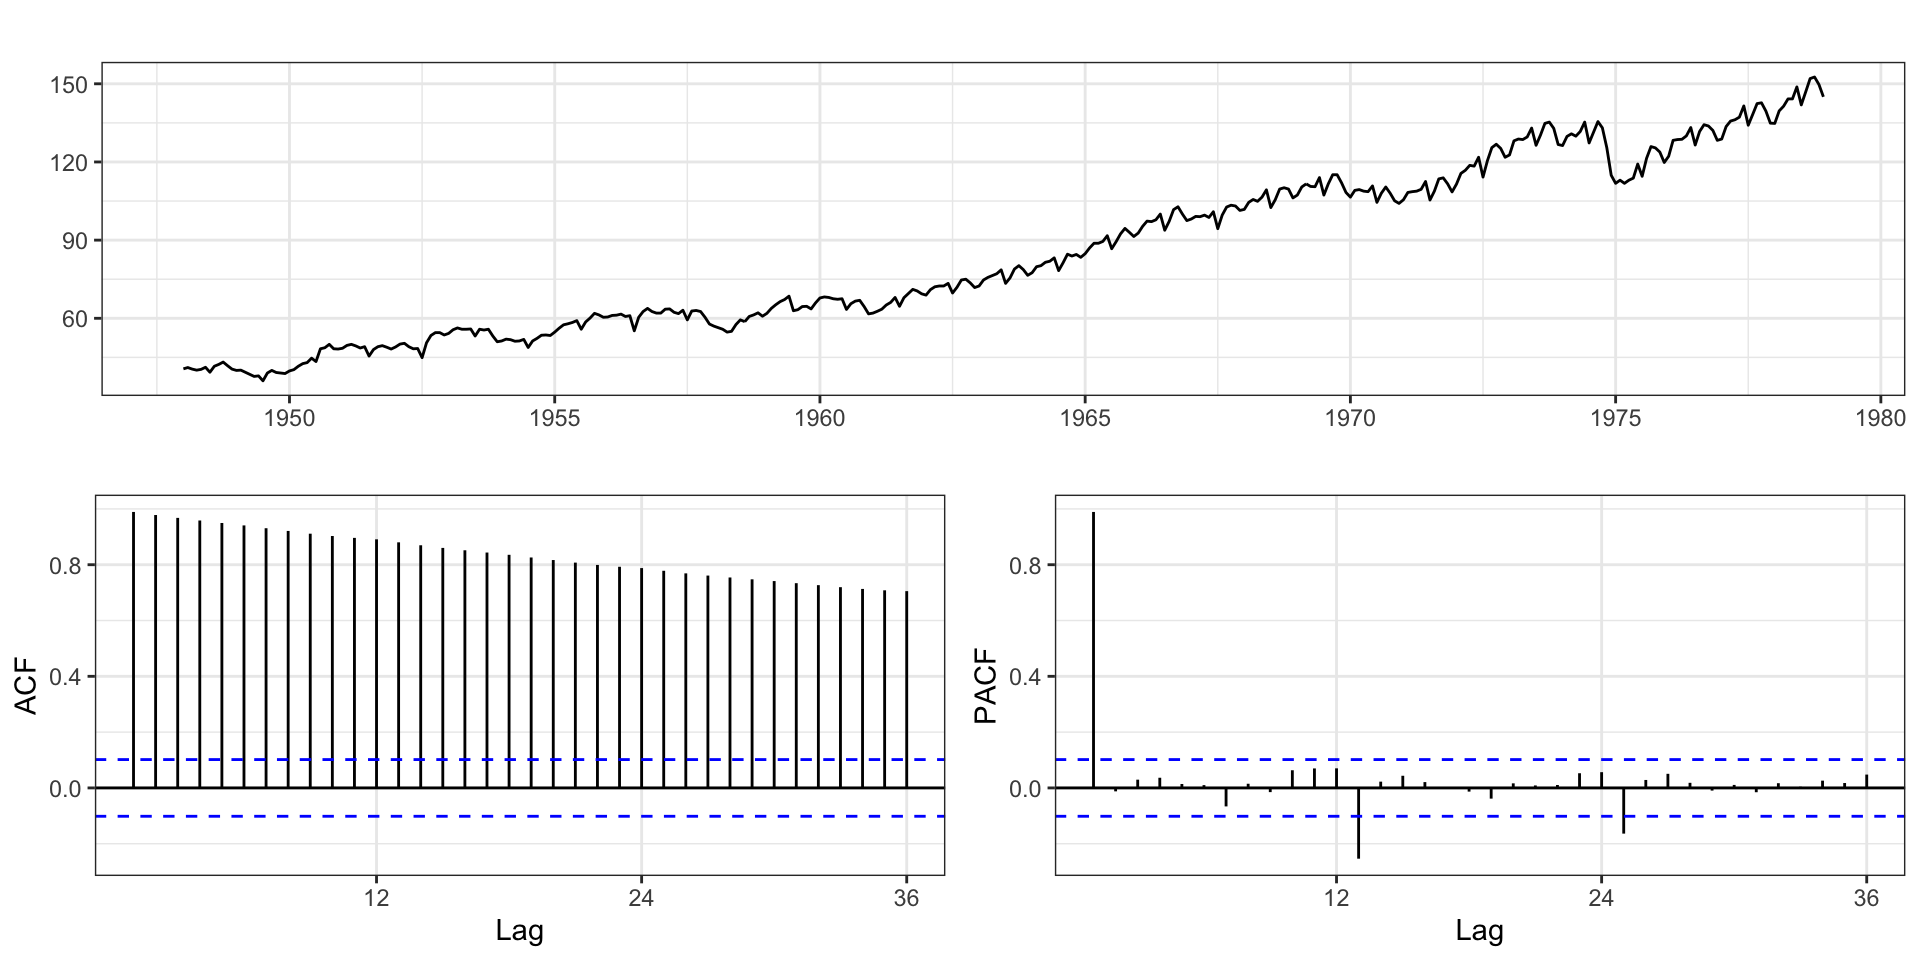
\includegraphics[width=\textwidth]{Lec11_files/figure-beamer/unnamed-chunk-15-1} \end{center}

\end{frame}

\begin{frame}[fragile]{Hannan-Rissanen - Step 3}
\protect\hypertarget{hannan-rissanen---step-3}{}

\scriptoutput

\begin{Shaded}
\begin{Highlighting}[]
\NormalTok{d =}\StringTok{ }\KeywordTok{data_frame}\NormalTok{(}
  \DataTypeTok{y =}\NormalTok{ y }\OperatorTok\StringTok{ }\KeywordTok{strip_attrs}\NormalTok{(), }
  \DataTypeTok{w_hat1 =}\NormalTok{ ar}\OperatorTok{$}\NormalTok{resid }\OperatorTok\StringTok{ }\KeywordTok{strip_attrs}\NormalTok{()}
\NormalTok{)}

\NormalTok{(}\DataTypeTok{lm1 =} \KeywordTok{lm}\NormalTok{(y }\OperatorTok{~}\StringTok{ }\KeywordTok{lag}\NormalTok{(y,}\DecValTok{1}\NormalTok{) }\OperatorTok{+}\StringTok{ }\KeywordTok{lag}\NormalTok{(y,}\DecValTok{2}\NormalTok{) }\OperatorTok{+}\StringTok{ }\KeywordTok{lag}\NormalTok{(w_hat1,}\DecValTok{1}\NormalTok{) }\OperatorTok{+}\StringTok{ }\KeywordTok{lag}\NormalTok{(w_hat1,}\DecValTok{2}\NormalTok{), }\DataTypeTok{data=}\NormalTok{d)) }\OperatorTok
\StringTok{  }\KeywordTok{summary}\NormalTok{()}
\CommentTok{## }
\CommentTok{## Call:}
\CommentTok{## lm(formula = y ~ lag(y, 1) + lag(y, 2) + lag(w_hat1, 1) + lag(w_hat1, }
\CommentTok{##     2), data = d)}
\CommentTok{## }
\CommentTok{## Residuals:}
\CommentTok{##      Min       1Q   Median       3Q      Max }
\CommentTok{## -2.62536 -0.59631  0.00282  0.69023  3.02714 }
\CommentTok{## }
\CommentTok{## Coefficients:}
\CommentTok{##                Estimate Std. Error t value Pr(>|t|)    }
\CommentTok{## (Intercept)     0.01405    0.04390   0.320    0.749    }
\CommentTok{## lag(y, 1)       1.31110    0.06062  21.629  < 2e-16 ***}
\CommentTok{## lag(y, 2)      -0.50714    0.05227  -9.702  < 2e-16 ***}
\CommentTok{## lag(w_hat1, 1)  0.50136    0.07587   6.608 1.01e-10 ***}
\CommentTok{## lag(w_hat1, 2)  0.15136    0.07567   2.000    0.046 *  }
\CommentTok{## ---}
\CommentTok{## Signif. codes:  0 '***' 0.001 '**' 0.01 '*' 0.05 '.' 0.1 ' ' 1}
\CommentTok{## }
\CommentTok{## Residual standard error: 0.9792 on 493 degrees of freedom}
\CommentTok{##   (2 observations deleted due to missingness)}
\CommentTok{## Multiple R-squared:  0.9258, Adjusted R-squared:  0.9252 }
\CommentTok{## F-statistic:  1537 on 4 and 493 DF,  p-value: < 2.2e-16}
\end{Highlighting}
\end{Shaded}

\end{frame}

\begin{frame}[fragile]{Hannan-Rissanen - Step 4.1}
\protect\hypertarget{hannan-rissanen---step-4.1}{}

\scriptoutput

\begin{Shaded}
\begin{Highlighting}[]
\NormalTok{d =}\StringTok{ }\NormalTok{modelr}\OperatorTok{::}\KeywordTok{add_residuals}\NormalTok{(d,lm1,}\StringTok{"w_hat2"}\NormalTok{)}

\NormalTok{(}\DataTypeTok{lm2 =} \KeywordTok{lm}\NormalTok{(y }\OperatorTok{~}\StringTok{ }\KeywordTok{lag}\NormalTok{(y,}\DecValTok{1}\NormalTok{) }\OperatorTok{+}\StringTok{ }\KeywordTok{lag}\NormalTok{(y,}\DecValTok{2}\NormalTok{) }\OperatorTok{+}\StringTok{ }\KeywordTok{lag}\NormalTok{(w_hat2,}\DecValTok{1}\NormalTok{) }\OperatorTok{+}\StringTok{ }\KeywordTok{lag}\NormalTok{(w_hat2,}\DecValTok{2}\NormalTok{), }\DataTypeTok{data=}\NormalTok{d)) }\OperatorTok
\StringTok{  }\KeywordTok{summary}\NormalTok{()}
\CommentTok{## }
\CommentTok{## Call:}
\CommentTok{## lm(formula = y ~ lag(y, 1) + lag(y, 2) + lag(w_hat2, 1) + lag(w_hat2, }
\CommentTok{##     2), data = d)}
\CommentTok{## }
\CommentTok{## Residuals:}
\CommentTok{##      Min       1Q   Median       3Q      Max }
\CommentTok{## -2.48938 -0.63467 -0.02144  0.64875  3.06169 }
\CommentTok{## }
\CommentTok{## Coefficients:}
\CommentTok{##                Estimate Std. Error t value Pr(>|t|)    }
\CommentTok{## (Intercept)     0.01732    0.04379   0.396   0.6926    }
\CommentTok{## lag(y, 1)       1.28435    0.06181  20.780  < 2e-16 ***}
\CommentTok{## lag(y, 2)      -0.48458    0.05322  -9.106  < 2e-16 ***}
\CommentTok{## lag(w_hat2, 1)  0.52941    0.07545   7.017 7.58e-12 ***}
\CommentTok{## lag(w_hat2, 2)  0.17436    0.07553   2.308   0.0214 *  }
\CommentTok{## ---}
\CommentTok{## Signif. codes:  0 '***' 0.001 '**' 0.01 '*' 0.05 '.' 0.1 ' ' 1}
\CommentTok{## }
\CommentTok{## Residual standard error: 0.9748 on 491 degrees of freedom}
\CommentTok{##   (4 observations deleted due to missingness)}
\CommentTok{## Multiple R-squared:  0.9267, Adjusted R-squared:  0.9261 }
\CommentTok{## F-statistic:  1553 on 4 and 491 DF,  p-value: < 2.2e-16}
\end{Highlighting}
\end{Shaded}

\end{frame}

\begin{frame}[fragile]{Hannan-Rissanen - Step 4.2}
\protect\hypertarget{hannan-rissanen---step-4.2}{}

\scriptoutput

\begin{Shaded}
\begin{Highlighting}[]
\NormalTok{d =}\StringTok{ }\NormalTok{modelr}\OperatorTok{::}\KeywordTok{add_residuals}\NormalTok{(d,lm2,}\StringTok{"w_hat3"}\NormalTok{)}

\NormalTok{(}\DataTypeTok{lm3 =} \KeywordTok{lm}\NormalTok{(y }\OperatorTok{~}\StringTok{ }\KeywordTok{lag}\NormalTok{(y,}\DecValTok{1}\NormalTok{) }\OperatorTok{+}\StringTok{ }\KeywordTok{lag}\NormalTok{(y,}\DecValTok{2}\NormalTok{) }\OperatorTok{+}\StringTok{ }\KeywordTok{lag}\NormalTok{(w_hat3,}\DecValTok{1}\NormalTok{) }\OperatorTok{+}\StringTok{ }\KeywordTok{lag}\NormalTok{(w_hat3,}\DecValTok{2}\NormalTok{), }\DataTypeTok{data=}\NormalTok{d)) }\OperatorTok
\StringTok{  }\KeywordTok{summary}\NormalTok{()}
\CommentTok{## }
\CommentTok{## Call:}
\CommentTok{## lm(formula = y ~ lag(y, 1) + lag(y, 2) + lag(w_hat3, 1) + lag(w_hat3, }
\CommentTok{##     2), data = d)}
\CommentTok{## }
\CommentTok{## Residuals:}
\CommentTok{##      Min       1Q   Median       3Q      Max }
\CommentTok{## -2.58530 -0.61844 -0.03113  0.66855  2.94198 }
\CommentTok{## }
\CommentTok{## Coefficients:}
\CommentTok{##                Estimate Std. Error t value Pr(>|t|)    }
\CommentTok{## (Intercept)     0.01411    0.04373   0.323  0.74712    }
\CommentTok{## lag(y, 1)       1.26447    0.06200  20.395  < 2e-16 ***}
\CommentTok{## lag(y, 2)      -0.46888    0.05335  -8.788  < 2e-16 ***}
\CommentTok{## lag(w_hat3, 1)  0.55598    0.07631   7.285 1.29e-12 ***}
\CommentTok{## lag(w_hat3, 2)  0.20607    0.07650   2.694  0.00731 ** }
\CommentTok{## ---}
\CommentTok{## Signif. codes:  0 '***' 0.001 '**' 0.01 '*' 0.05 '.' 0.1 ' ' 1}
\CommentTok{## }
\CommentTok{## Residual standard error: 0.9714 on 489 degrees of freedom}
\CommentTok{##   (6 observations deleted due to missingness)}
\CommentTok{## Multiple R-squared:  0.9274, Adjusted R-squared:  0.9268 }
\CommentTok{## F-statistic:  1562 on 4 and 489 DF,  p-value: < 2.2e-16}
\end{Highlighting}
\end{Shaded}

\end{frame}

\begin{frame}[fragile]{Hannan-Rissanen - Step 4.3}
\protect\hypertarget{hannan-rissanen---step-4.3}{}

\scriptoutput

\begin{Shaded}
\begin{Highlighting}[]
\NormalTok{d =}\StringTok{ }\NormalTok{modelr}\OperatorTok{::}\KeywordTok{add_residuals}\NormalTok{(d,lm3,}\StringTok{"w_hat4"}\NormalTok{)}

\NormalTok{(}\DataTypeTok{lm4 =} \KeywordTok{lm}\NormalTok{(y }\OperatorTok{~}\StringTok{ }\KeywordTok{lag}\NormalTok{(y,}\DecValTok{1}\NormalTok{) }\OperatorTok{+}\StringTok{ }\KeywordTok{lag}\NormalTok{(y,}\DecValTok{2}\NormalTok{) }\OperatorTok{+}\StringTok{ }\KeywordTok{lag}\NormalTok{(w_hat4,}\DecValTok{1}\NormalTok{) }\OperatorTok{+}\StringTok{ }\KeywordTok{lag}\NormalTok{(w_hat4,}\DecValTok{2}\NormalTok{), }\DataTypeTok{data=}\NormalTok{d)) }\OperatorTok
\StringTok{  }\KeywordTok{summary}\NormalTok{()}
\CommentTok{## }
\CommentTok{## Call:}
\CommentTok{## lm(formula = y ~ lag(y, 1) + lag(y, 2) + lag(w_hat4, 1) + lag(w_hat4, }
\CommentTok{##     2), data = d)}
\CommentTok{## }
\CommentTok{## Residuals:}
\CommentTok{##      Min       1Q   Median       3Q      Max }
\CommentTok{## -2.47793 -0.62637 -0.02602  0.67771  3.01388 }
\CommentTok{## }
\CommentTok{## Coefficients:}
\CommentTok{##                 Estimate Std. Error t value Pr(>|t|)    }
\CommentTok{## (Intercept)     0.006615   0.043826   0.151   0.8801    }
\CommentTok{## lag(y, 1)       1.270581   0.062110  20.457  < 2e-16 ***}
\CommentTok{## lag(y, 2)      -0.474331   0.053406  -8.882  < 2e-16 ***}
\CommentTok{## lag(w_hat4, 1)  0.546706   0.076724   7.126 3.75e-12 ***}
\CommentTok{## lag(w_hat4, 2)  0.195828   0.077098   2.540   0.0114 *  }
\CommentTok{## ---}
\CommentTok{## Signif. codes:  0 '***' 0.001 '**' 0.01 '*' 0.05 '.' 0.1 ' ' 1}
\CommentTok{## }
\CommentTok{## Residual standard error: 0.9719 on 487 degrees of freedom}
\CommentTok{##   (8 observations deleted due to missingness)}
\CommentTok{## Multiple R-squared:  0.9269, Adjusted R-squared:  0.9263 }
\CommentTok{## F-statistic:  1543 on 4 and 487 DF,  p-value: < 2.2e-16}
\end{Highlighting}
\end{Shaded}

\end{frame}

\begin{frame}[fragile]{Hannan-Rissanen - Step 4.4}
\protect\hypertarget{hannan-rissanen---step-4.4}{}

\scriptoutput

\begin{Shaded}
\begin{Highlighting}[]
\NormalTok{d =}\StringTok{ }\NormalTok{modelr}\OperatorTok{::}\KeywordTok{add_residuals}\NormalTok{(d,lm4,}\StringTok{"w_hat5"}\NormalTok{)}

\NormalTok{(}\DataTypeTok{lm5 =} \KeywordTok{lm}\NormalTok{(y }\OperatorTok{~}\StringTok{ }\KeywordTok{lag}\NormalTok{(y,}\DecValTok{1}\NormalTok{) }\OperatorTok{+}\StringTok{ }\KeywordTok{lag}\NormalTok{(y,}\DecValTok{2}\NormalTok{) }\OperatorTok{+}\StringTok{ }\KeywordTok{lag}\NormalTok{(w_hat5,}\DecValTok{1}\NormalTok{) }\OperatorTok{+}\StringTok{ }\KeywordTok{lag}\NormalTok{(w_hat5,}\DecValTok{2}\NormalTok{), }\DataTypeTok{data=}\NormalTok{d)) }\OperatorTok
\StringTok{  }\KeywordTok{summary}\NormalTok{()}
\CommentTok{## }
\CommentTok{## Call:}
\CommentTok{## lm(formula = y ~ lag(y, 1) + lag(y, 2) + lag(w_hat5, 1) + lag(w_hat5, }
\CommentTok{##     2), data = d)}
\CommentTok{## }
\CommentTok{## Residuals:}
\CommentTok{##      Min       1Q   Median       3Q      Max }
\CommentTok{## -2.52482 -0.61986 -0.01755  0.65755  3.01411 }
\CommentTok{## }
\CommentTok{## Coefficients:}
\CommentTok{##                 Estimate Std. Error t value Pr(>|t|)    }
\CommentTok{## (Intercept)     0.002506   0.043950   0.057  0.95456    }
\CommentTok{## lag(y, 1)       1.261588   0.062919  20.051  < 2e-16 ***}
\CommentTok{## lag(y, 2)      -0.468001   0.053869  -8.688  < 2e-16 ***}
\CommentTok{## lag(w_hat5, 1)  0.555958   0.077424   7.181 2.62e-12 ***}
\CommentTok{## lag(w_hat5, 2)  0.202817   0.077796   2.607  0.00941 ** }
\CommentTok{## ---}
\CommentTok{## Signif. codes:  0 '***' 0.001 '**' 0.01 '*' 0.05 '.' 0.1 ' ' 1}
\CommentTok{## }
\CommentTok{## Residual standard error: 0.9728 on 485 degrees of freedom}
\CommentTok{##   (10 observations deleted due to missingness)}
\CommentTok{## Multiple R-squared:  0.9261, Adjusted R-squared:  0.9255 }
\CommentTok{## F-statistic:  1519 on 4 and 485 DF,  p-value: < 2.2e-16}
\end{Highlighting}
\end{Shaded}

\end{frame}

\begin{frame}[fragile]{RMSEs}
\protect\hypertarget{rmses}{}

\begin{Shaded}
\begin{Highlighting}[]
\NormalTok{modelr}\OperatorTok{::}\KeywordTok{rmse}\NormalTok{(lm1, }\DataTypeTok{data =}\NormalTok{ d)}
\CommentTok{## [1] 0.9743158}

\NormalTok{modelr}\OperatorTok{::}\KeywordTok{rmse}\NormalTok{(lm2, }\DataTypeTok{data =}\NormalTok{ d)}
\CommentTok{## [1] 0.9698713}

\NormalTok{modelr}\OperatorTok{::}\KeywordTok{rmse}\NormalTok{(lm3, }\DataTypeTok{data =}\NormalTok{ d)}
\CommentTok{## [1] 0.9665092}

\NormalTok{modelr}\OperatorTok{::}\KeywordTok{rmse}\NormalTok{(lm4, }\DataTypeTok{data =}\NormalTok{ d)}
\CommentTok{## [1] 0.9669626}

\NormalTok{modelr}\OperatorTok{::}\KeywordTok{rmse}\NormalTok{(lm5, }\DataTypeTok{data =}\NormalTok{ d)}
\CommentTok{## [1] 0.9678429}
\end{Highlighting}
\end{Shaded}

\end{frame}

\begin{frame}[fragile]{JAGS - Model}
\protect\hypertarget{jags---model}{}

\tinyoutput

\begin{Shaded}
\begin{Highlighting}[]
\NormalTok{arma22_model =}\StringTok{ "model\{}
\StringTok{# Likelihood}
\StringTok{  for (t in 1:length(y)) \{}
\StringTok{    y[t] ~ dnorm(mu[t], 1/sigma2_e)}
\StringTok{  \}                                   }

\StringTok{  mu[1] = phi[1] * y_0  + phi[2] * y_n1 + w[1] + theta[1]*w_0  + theta[2]*w_n1}
\StringTok{  mu[2] = phi[1] * y[1] + phi[2] * y_0  + w[2] + theta[1]*w[1] + theta[2]*w_0   }

\StringTok{  for (t in 3:length(y)) \{ }
\StringTok{    mu[t] = phi[1] * y[t-1] + phi[2] * y[t-2] + w[t] + theta[1] * w[t-1] + theta[2] * w[t-2]}
\StringTok{  \}}
\StringTok{  }
\StringTok{# Priors}
\StringTok{  for(t in 1:length(y))\{}
\StringTok{    w[t] ~ dnorm(0,1/sigma2_w)}
\StringTok{  \}}

\StringTok{  sigma2_w = 1/tau_w; tau_w ~ dgamma(0.001, 0.001) }
\StringTok{  sigma2_e = 1/tau_e; tau_e ~ dgamma(0.001, 0.001) }
\StringTok{  for(i in 1:2) \{}
\StringTok{    phi[i] ~ dnorm(0,1)}
\StringTok{    theta[i] ~ dnorm(0,1)}
\StringTok{  \}}

\StringTok{# Latent errors and series values}
\StringTok{  w_0  ~ dnorm(0, 1/sigma2_w)}
\StringTok{  w_n1 ~ dnorm(0, 1/sigma2_w)}
\StringTok{  y_0  ~ dnorm(0, 1/4)}
\StringTok{  y_n1 ~ dnorm(0, 1/4)}
\StringTok{\}"}
\end{Highlighting}
\end{Shaded}

\end{frame}

\begin{frame}{JAGS - Fit}
\protect\hypertarget{jags---fit}{}

\begin{center}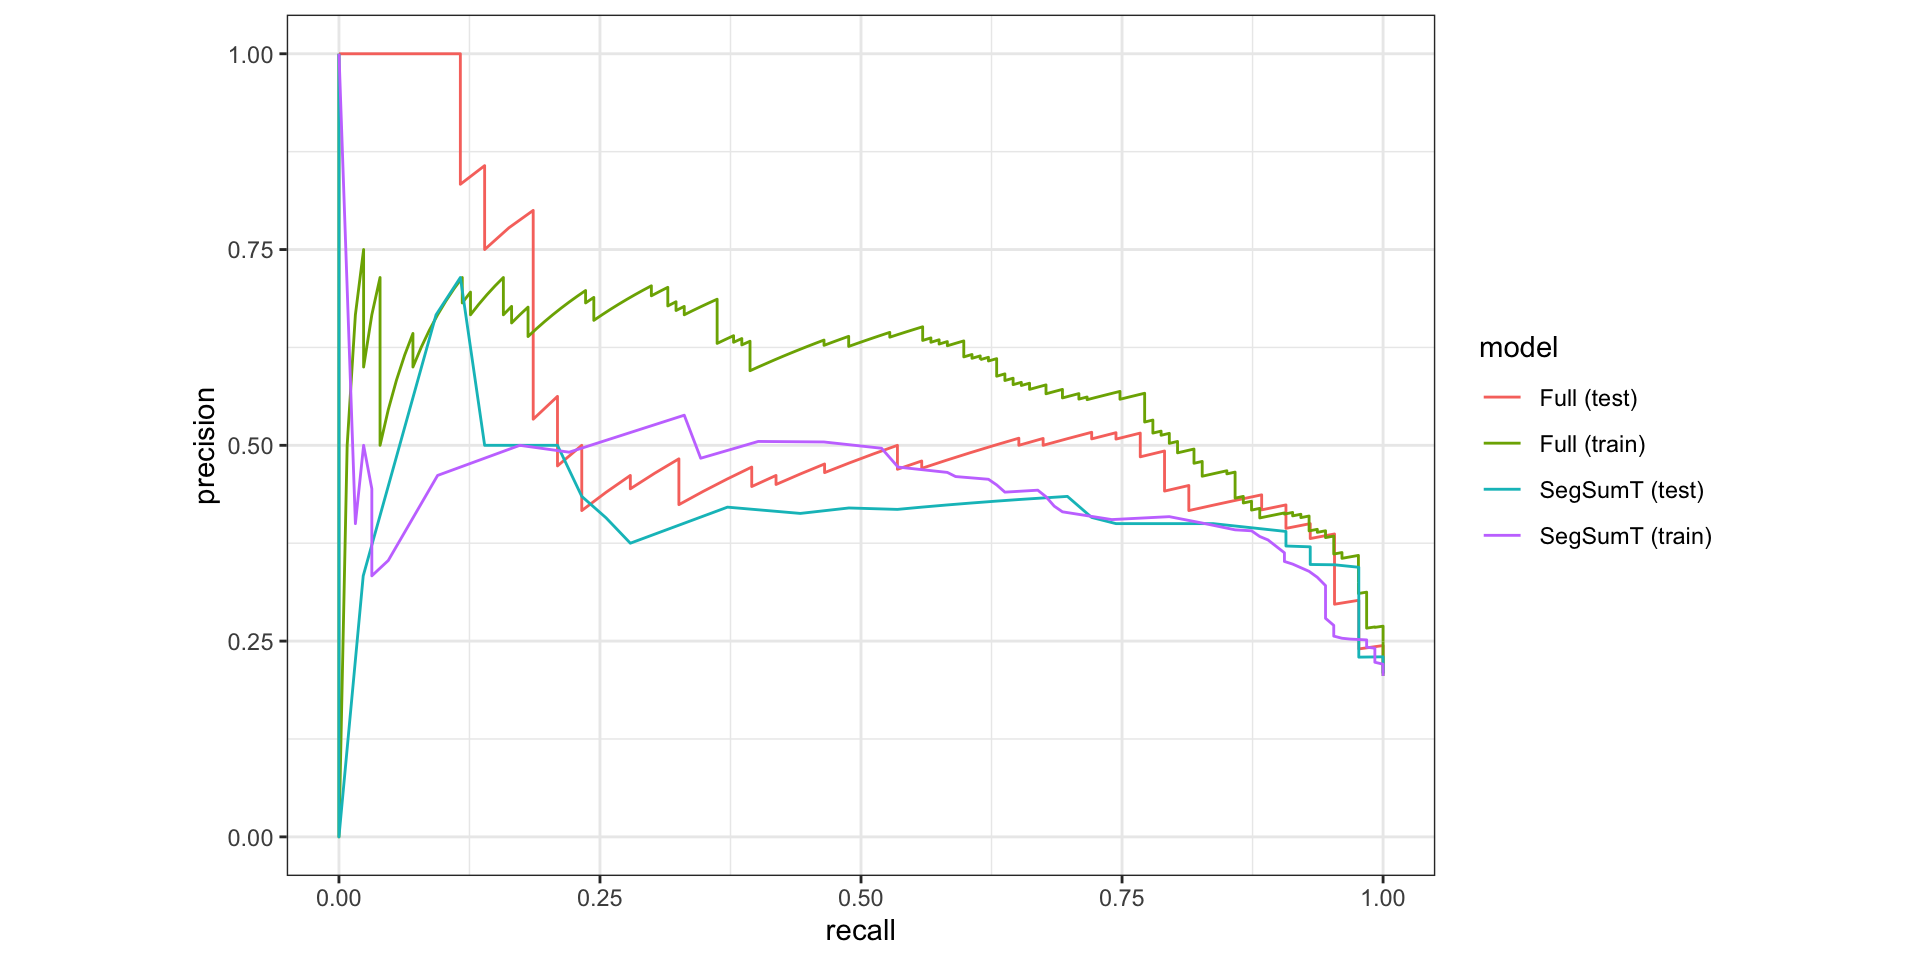
\includegraphics[width=\textwidth]{Lec11_files/figure-beamer/unnamed-chunk-24-1} \end{center}

\end{frame}

\begin{frame}{JAGS - Posteriors}
\protect\hypertarget{jags---posteriors}{}

\begin{center}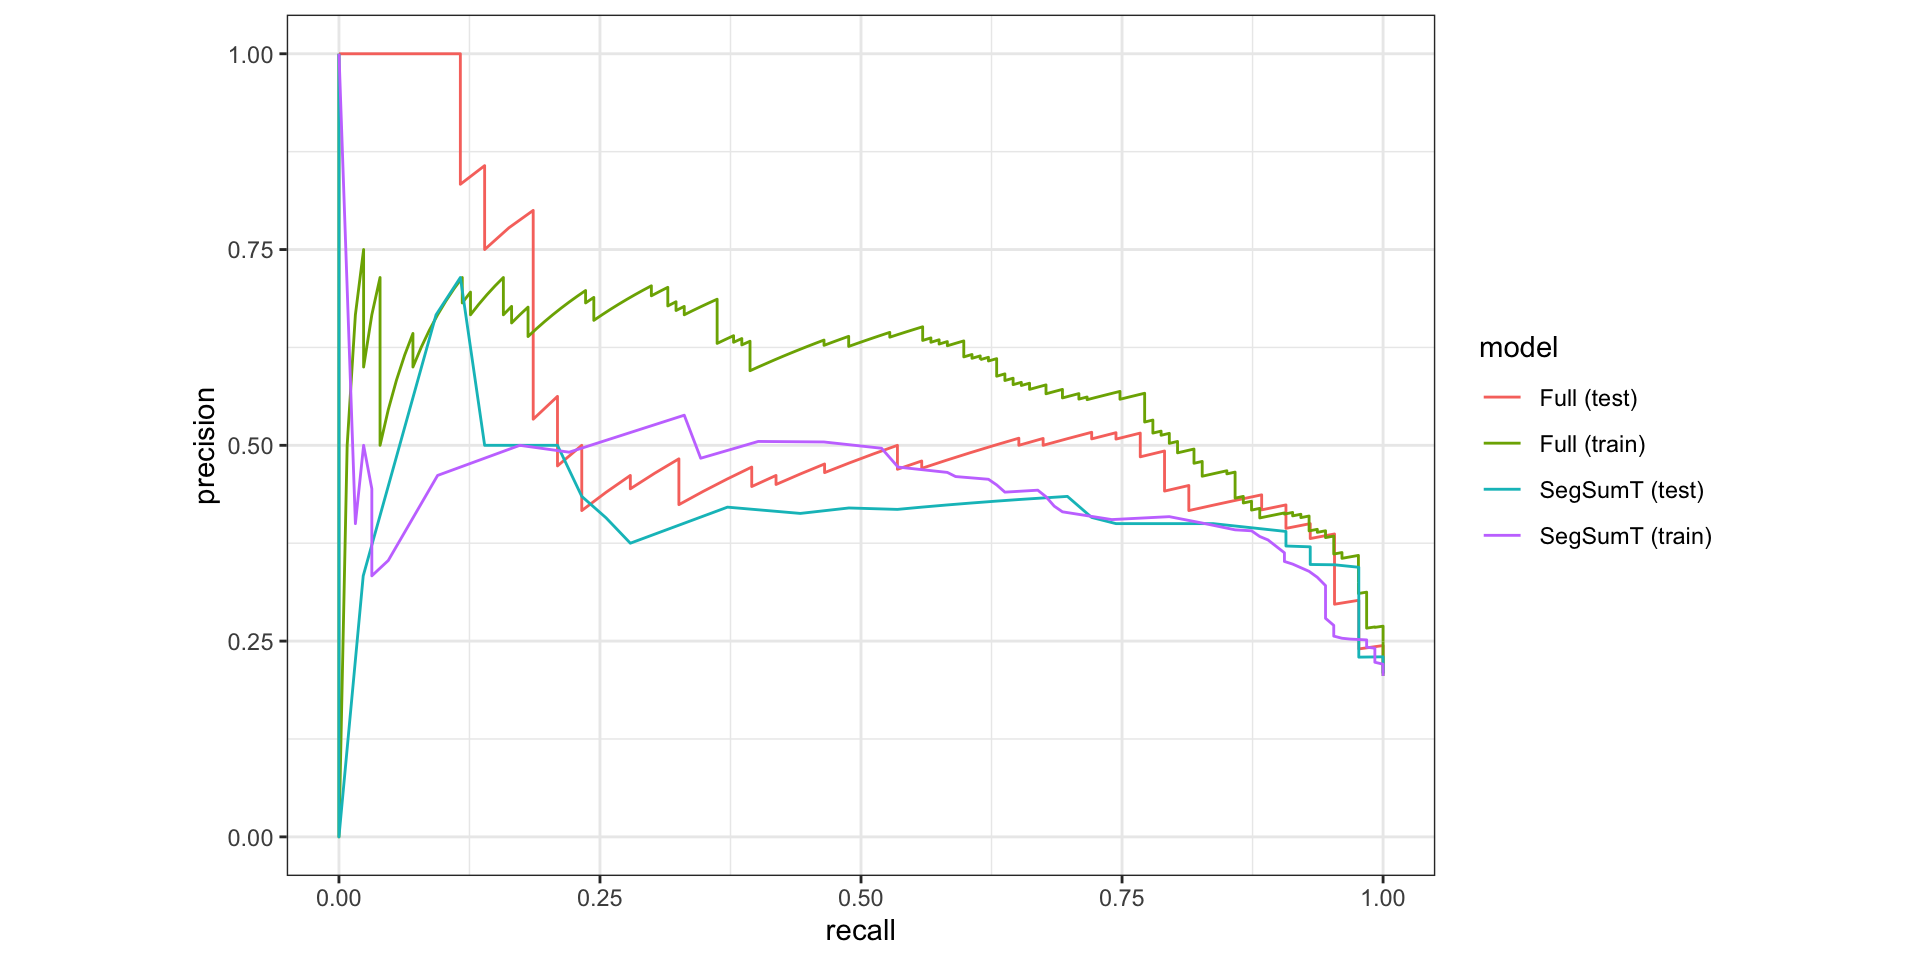
\includegraphics[width=\textwidth]{Lec11_files/figure-beamer/unnamed-chunk-25-1} \end{center}

\end{frame}

\begin{frame}[fragile]{Using \texttt{brms}}
\protect\hypertarget{using-brms}{}

\begin{Shaded}
\begin{Highlighting}[]
\KeywordTok{library}\NormalTok{(brms)}
\NormalTok{b =}\StringTok{ }\KeywordTok{brm}\NormalTok{(y}\OperatorTok{~}\DecValTok{1}\NormalTok{, }\DataTypeTok{data =}\NormalTok{ d, }\DataTypeTok{autocor =} \KeywordTok{cor_arma}\NormalTok{(}\DataTypeTok{p=}\DecValTok{2}\NormalTok{,}\DataTypeTok{q=}\DecValTok{2}\NormalTok{), }\DataTypeTok{chains =} \DecValTok{2}\NormalTok{)}
\end{Highlighting}
\end{Shaded}

\tinyoutput

\begin{Shaded}
\begin{Highlighting}[]
\CommentTok{## Compiling the C++ model}
\CommentTok{## Start sampling}
\CommentTok{##}
\CommentTok{## SAMPLING FOR MODEL '90ac5aa650e5db28db8b9b83a5eb3c07' NOW (CHAIN 1).}
\CommentTok{## }
\CommentTok{## Gradient evaluation took 0.001742 seconds}
\CommentTok{## 1000 transitions using 10 leapfrog steps per transition would take 17.42 seconds.}
\CommentTok{## Adjust your expectations accordingly!}
\CommentTok{## }
\CommentTok{## Iteration:    1 / 2000 [  0%]  (Warmup)}
\CommentTok{## Iteration:  200 / 2000 [ 10%]  (Warmup)}
\CommentTok{## Iteration:  400 / 2000 [ 20%]  (Warmup)}
\CommentTok{## Iteration:  600 / 2000 [ 30%]  (Warmup)}
\CommentTok{## Iteration:  800 / 2000 [ 40%]  (Warmup)}
\CommentTok{## Iteration: 1000 / 2000 [ 50%]  (Warmup)}
\CommentTok{## Iteration: 1001 / 2000 [ 50%]  (Sampling)}
\CommentTok{## Iteration: 1001 / 2000 [ 50%]  (Sampling)}
\CommentTok{## Iteration: 1200 / 2000 [ 60%]  (Sampling)}
\CommentTok{## Iteration: 1400 / 2000 [ 70%]  (Sampling)}
\CommentTok{## Iteration: 1600 / 2000 [ 80%]  (Sampling)}
\CommentTok{## Iteration: 1800 / 2000 [ 90%]  (Sampling)}
\CommentTok{## Iteration: 2000 / 2000 [100%]  (Sampling)}
\CommentTok{## }
\CommentTok{##  Elapsed Time: 13.2358 seconds (Warm-up)}
\CommentTok{##                9.79355 seconds (Sampling)}
\CommentTok{##                23.0293 seconds (Total)}
\end{Highlighting}
\end{Shaded}

\end{frame}

\begin{frame}{BRMS - Chains}
\protect\hypertarget{brms---chains}{}

\begin{center}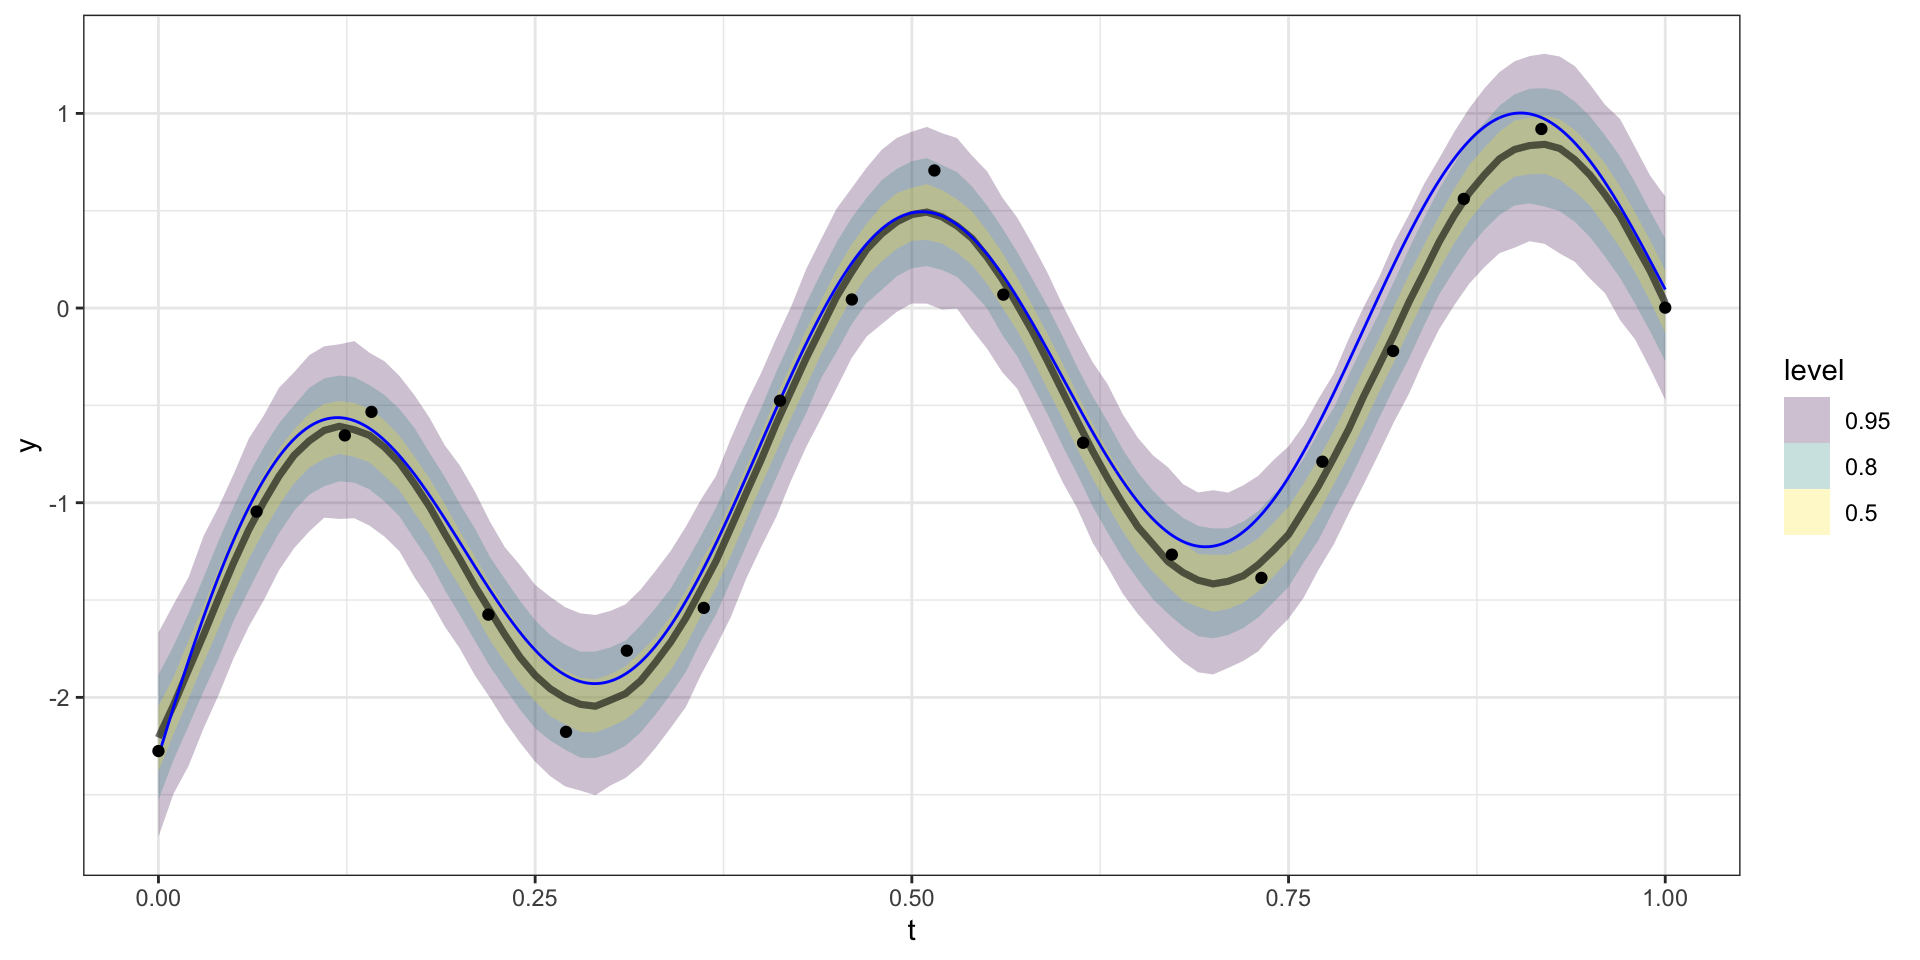
\includegraphics[width=\textwidth]{Lec11_files/figure-beamer/unnamed-chunk-27-1} \end{center}

\end{frame}

\begin{frame}{BRMS - Posteriors}
\protect\hypertarget{brms---posteriors}{}

\begin{center}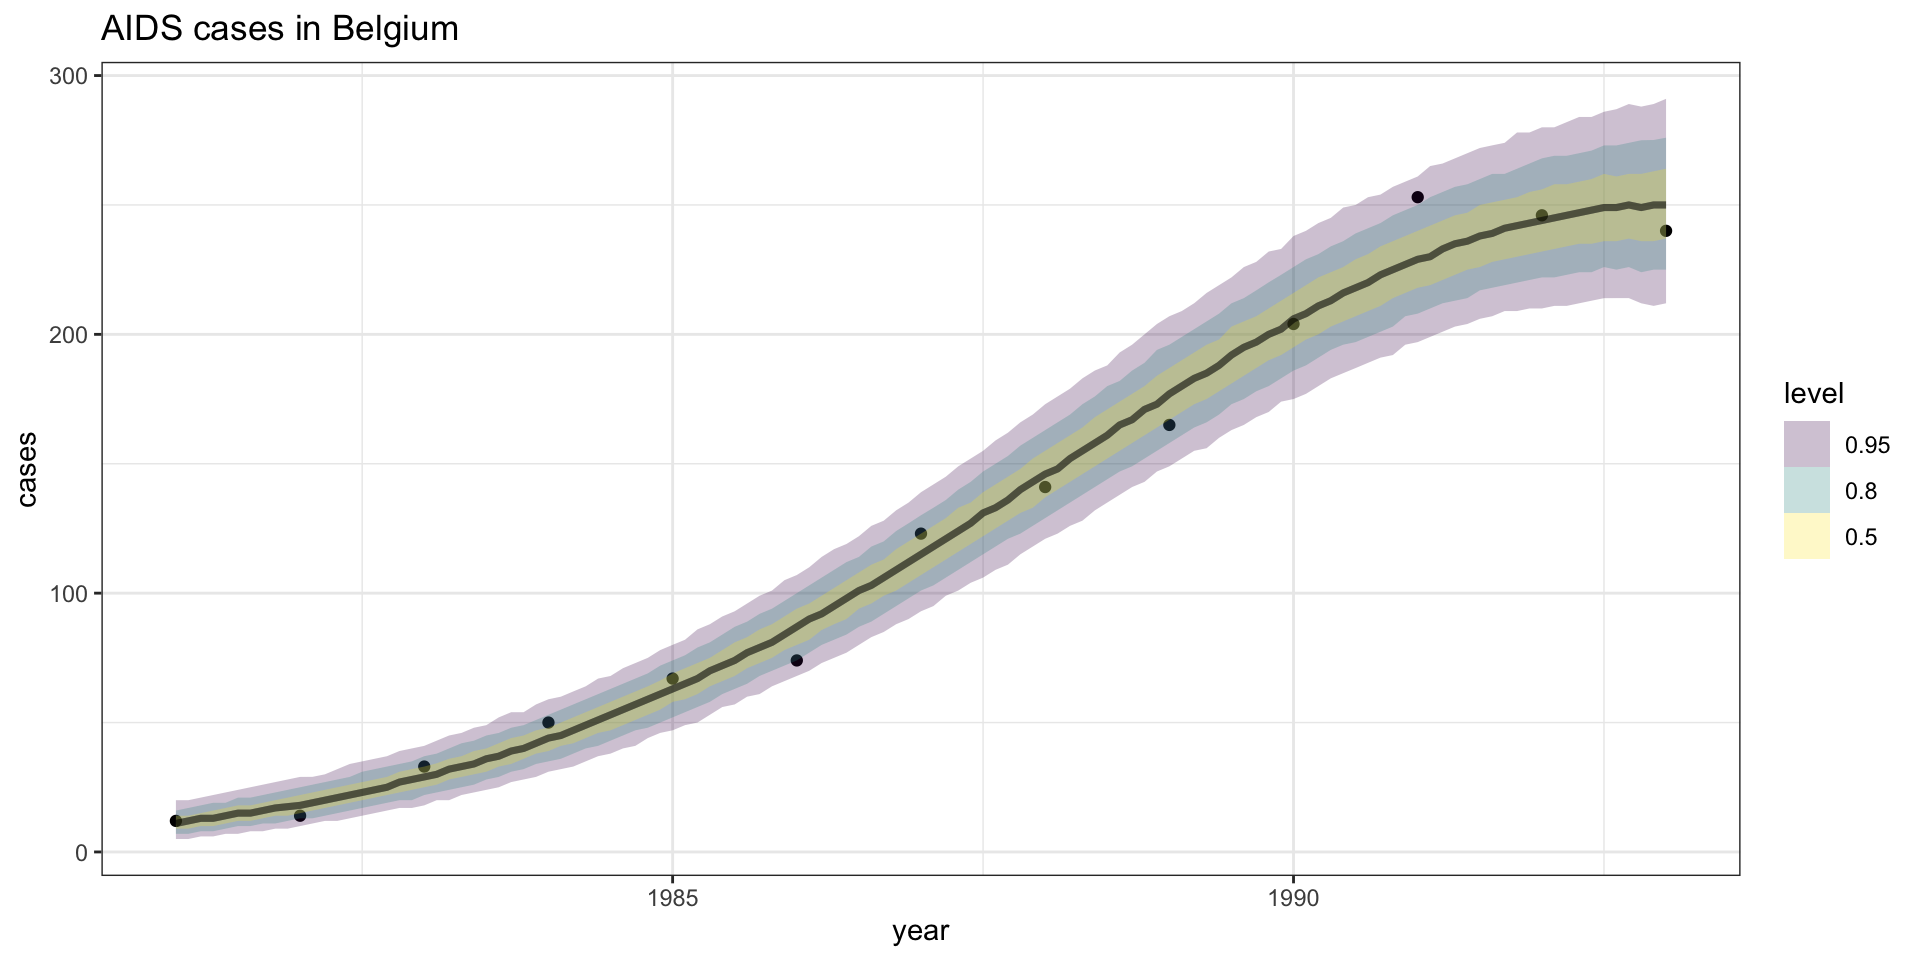
\includegraphics[width=\textwidth]{Lec11_files/figure-beamer/unnamed-chunk-28-1} \end{center}

\end{frame}

\begin{frame}{BRMS - Predictions}
\protect\hypertarget{brms---predictions}{}

\begin{center}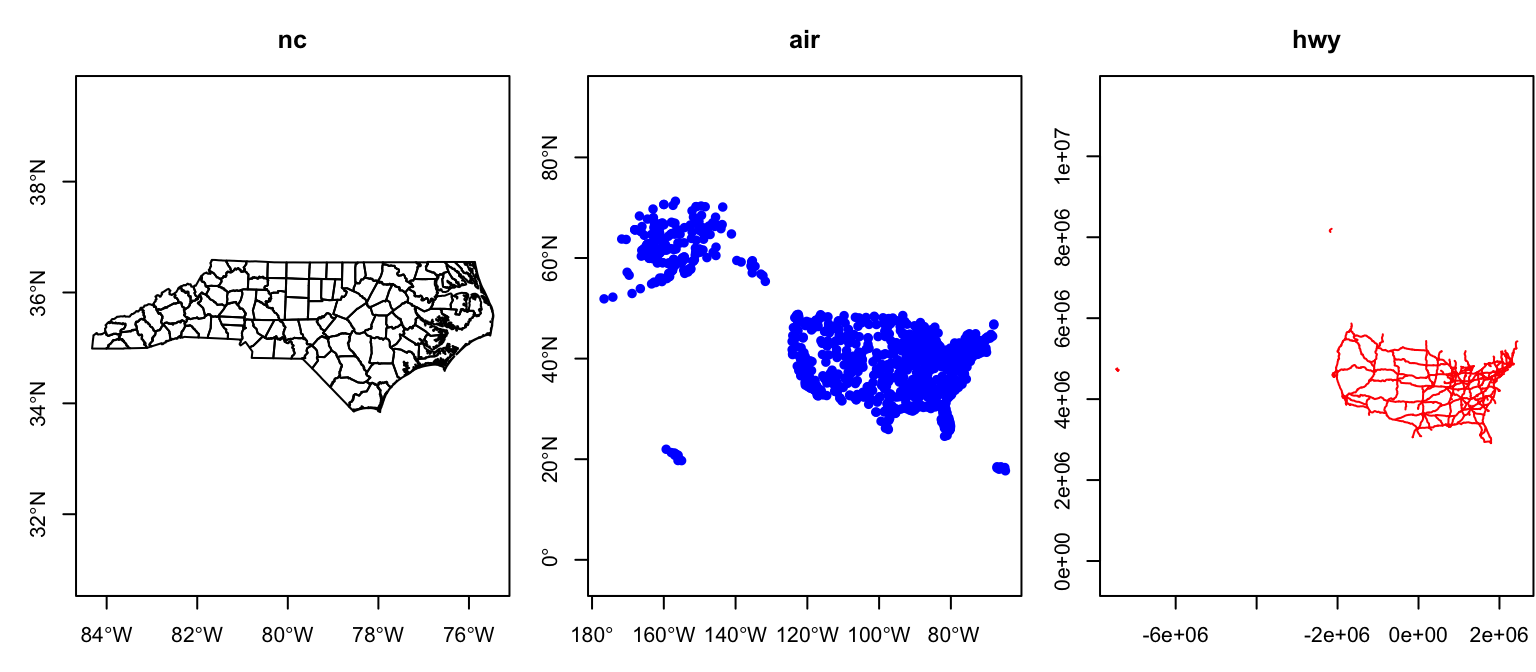
\includegraphics[width=\textwidth]{Lec11_files/figure-beamer/unnamed-chunk-29-1} \end{center}

\end{frame}

\begin{frame}[fragile]{BRMS - Stancode}
\protect\hypertarget{brms---stancode}{}

\tinyoutput

\begin{Shaded}
\begin{Highlighting}[]
\KeywordTok{stancode}\NormalTok{(b)}
\CommentTok{## // generated with brms 2.5.0}
\CommentTok{## functions \{ }
\CommentTok{## \} }
\CommentTok{## data \{ }
\CommentTok{##   int<lower=1> N;  // total number of observations }
\CommentTok{##   vector[N] Y;  // response variable }
\CommentTok{##   // data needed for ARMA correlations }
\CommentTok{##   int<lower=0> Kar;  // AR order }
\CommentTok{##   int<lower=0> Kma;  // MA order }
\CommentTok{##   int<lower=0> J_lag[N]; }
\CommentTok{##   int prior_only;  // should the likelihood be ignored? }
\CommentTok{## \} }
\CommentTok{## transformed data \{ }
\CommentTok{##   int max_lag = max(Kar, Kma); }
\CommentTok{## \} }
\CommentTok{## parameters \{ }
\CommentTok{##   real temp_Intercept;  // temporary intercept }
\CommentTok{##   real<lower=0> sigma;  // residual SD }
\CommentTok{##   vector<lower=-1,upper=1>[Kar] ar;  // autoregressive effects }
\CommentTok{##   vector<lower=-1,upper=1>[Kma] ma;  // moving-average effects }
\CommentTok{## \} }
\CommentTok{## transformed parameters \{ }
\CommentTok{## \} }
\CommentTok{## model \{ }
\CommentTok{##   vector[N] mu = temp_Intercept + rep_vector(0, N);}
\CommentTok{##   // objects storing residuals }
\CommentTok{##   matrix[N, max_lag] E = rep_matrix(0, N, max_lag); }
\CommentTok{##   vector[N] e; }
\CommentTok{##   for (n in 1:N) \{ }
\CommentTok{##     mu[n] += head(E[n], Kma) * ma;}
\CommentTok{##     // computation of ARMA correlations }
\CommentTok{##     e[n] = Y[n] - mu[n]; }
\CommentTok{##     for (i in 1:J_lag[n]) \{ }
\CommentTok{##       E[n + 1, i] = e[n + 1 - i]; }
\CommentTok{##     \} }
\CommentTok{##     mu[n] += head(E[n], Kar) * ar;}
\CommentTok{##   \} }
\CommentTok{##   // priors including all constants }
\CommentTok{##   target += student_t_lpdf(temp_Intercept | 3, 0, 10); }
\CommentTok{##   target += student_t_lpdf(sigma | 3, 0, 10)}
\CommentTok{##     - 1 * student_t_lccdf(0 | 3, 0, 10); }
\CommentTok{##   // likelihood including all constants }
\CommentTok{##   if (!prior_only) \{ }
\CommentTok{##     target += normal_lpdf(Y | mu, sigma);}
\CommentTok{##   \} }
\CommentTok{## \} }
\CommentTok{## generated quantities \{ }
\CommentTok{##   // actual population-level intercept }
\CommentTok{##   real b_Intercept = temp_Intercept; }
\CommentTok{## \}}
\end{Highlighting}
\end{Shaded}

\end{frame}

\end{document}
